\documentclass[12pt,letter]{article}
\usepackage[DIV=14,BCOR=2mm,headinclude=true,footinclude=false]{typearea}
\renewcommand{\baselinestretch}{1.5} 
\usepackage{latexsym}
\usepackage{amsmath}
%\usepackage{mathabx}

\usepackage{titlesec}
%\titleformat{\section}[block]{\color{blue}\Large\bfseries\filcenter}{}{1em}{}
%\titleformat{\subsection}[hang]{\bfseries}{}{1em}{}

%\usepackage{sectsty}
%\sectionfont{\centering}

\usepackage{pdflscape}

%\usepackage{MinionPro}
\usepackage{amssymb}

\usepackage{hyperref}
\usepackage{tikz}
\usepackage{verbatim}
\usepackage{natbib}
\usepackage{color, colortbl}
\usepackage{appendix}
\usepackage{amsmath,amsthm}

%\usepackage[]{figcaps}

\usepackage{wasysym}


\newcommand{\Rho}{\mathrm{R}}
\newcommand{\Kappa}{\mathrm{K}}
\newcommand{\Omicron}{\mathrm{O}}
\newcommand\omicron{o}

\usetikzlibrary{arrows,shapes}

\definecolor{Gray}{gray}{0.9}

\newtheorem{result}{Result}
\newtheorem{theorem}{Theorem}
\newtheorem*{theorem*}{Theorem}
\newtheorem{conjecture}{Conjecture}[section]
\newtheorem{corollary}{Corollary}[section]
\newtheorem{lemma}{Lemma}[section]
\newtheorem*{lemma*}{Lemma}
\newtheorem{proposition}{Proposition}[section]
\newtheorem{definition}{Definition}[section]
\newtheorem{assumption}{Assumption}[section]


\theoremstyle{definition}
\newtheorem{example}{Example}

\theoremstyle{remark}
\newtheorem*{remark}{Remark}

\theoremstyle{claim}
\newtheorem{claim}{Claim}


\pgfdeclarelayer{background}
\pgfsetlayers{background,main}

\tikzstyle{vertex}=[circle, draw
%,fill=black!25
,minimum size=12pt
,inner sep=0pt
]
\usetikzlibrary{decorations.pathreplacing}
\tikzstyle{selected vertex} = [vertex, fill=red!24]
%\tikzstyle{unknown vertex} = [vertex, fill=black!25]
\tikzstyle{unknown vertex} = [vertex, fill=white]
\tikzstyle{edge} = [draw,thick,-]
\tikzstyle{weight} = [font=\small]
\tikzstyle{selected edge} = [draw,line width=5pt,-,red!50]
\tikzstyle{ignored edge} = [draw,line width=5pt,-,black!20]
\newcommand{\bigtimes}{\mathbin{\tikz [x=1.4ex,y=1.4ex,line width=.2ex] \draw (0,0) -- (1,1) (0,1) -- (1,0);}}%


%\linespread{1.5}

\begin{document}
%\fontsize{12}{20pt}\selectfont

\title {Coordination in Social Networks: Communication by Actions}
\author {Chun-Ting Chen}
\date{July 30, 2019}
\maketitle

\begin{abstract}

%This paper studies a collective action problem in a setting of discounted repeated coordination games in which players know their neighbors'  inclination to participate as well as monitor their neighbors' past actions. I define \textit{strong connectedness} to characterize those states in which, for every two players who incline to participate, there is a path consisting of players with the same inclination to connect them.  Given that the networks are fixed, finite, connected, commonly known, undirected and without cycles, I show that if the priors have full support on the strong connectedness states, there is a (weak) sequential equilibrium in which the ex-post efficient outcome repeats after a finite time $T$ in the path when discount factor is sufficiently high. This equilibrium is constructive and does not depend on public or private signals other than players' actions.




\end{abstract}


\section{Introduction} 

%This paper studies collective actions in a setting of discounted repeated coordination games, where information and monitoring structures are modeled as networks. Players are uncertain about the states of nature but can observe their neighbors' actions. I would like to explore what kinds of networks can induce players to solve the underlying uncertainty in order to coordinate with the ex-post efficient outcome. Though the motive of this study is to understand the dynamic of social movements, a general interest centers on the collective action behaviors within social structures.
%
%Consider pro-democracy movements. Strong discontents overthrowing a regime may exist, but it is difficult to organized around these discontents because information about the existence of such discontents is not always transparent. For instance, in East Germany, the government had control over the electoral system and the mass media, and the eavesdropping by secret agents had impeded people from showing their discontents. As \citep{Karl-Dieter1993} or \citep{Chwe2000} have suggested, such discontents may be revealed only to someone whom you trust or have an intimate relationship with, but are hardly revealed publicly. This lack of common knowledge about the existence of strong discontent may impede people from conducting a one-shot uprising due to the fear of possible failure (e.g., \citep{Chwe2000} in proposing a static model to characterize the networks that provide common knowledge about peoples' discontents). However, an event may trigger a later event (e.g., \citep{Lohmann2011} in using informational cascade model to explain consecutive demonstrations in East Germany 1989-1991). When rebels are aware of the scale to transmit relevant information about the level of collective discontent through their actions, they might be willing to act although it might be at risk of facing failure. I view such risky actions as a part of an equilibrium strategy and the entire movement as a learning process. 
%
%
%
%
%Inspired by \citep{Chwe2000}, I model such dynamic collective action in the following way. Players repeatedly play a $k$-\textit{Threshold game} with a parameter $k$ in a network. There are two types of players located in the network, one we called them \textit{Rebel} and one we called them \textit{Inert}.  Players' types and their actions can be observed only by their neighbors. A Rebel has two actions, which are \textbf{revolt} or \textbf{stay} while an Inert has only one action, which is \textbf{stay}. A Rebel will get payoff as $1$ if he chooses \textbf{revolt} and more than $k$ players choose \textbf{revolt}; he will get payoff as $-1$ if he chooses \textbf{revolt} and less than $k$ players choose \textbf{revolt}; he will get payoff as $0$ if he chooses \textbf{stay}. An Inert will get payoff as $1$ if he chooses \textbf{stay}.
%
%Since a Rebel may not know how many Rebels exist in this world, Rebels' payoff structure captures the idea that \textbf{stay} is a safe arm and \textbf{revolt} is a risky arm. Given a common prior $\pi$ over players' types, players play this $k$-Threshold game infinitely repeatedly with a common discount factor $\delta$. Cheap talk is not allowed, no outside mechanism serves as an information sharing device. 
%
%Rebels then communicate with each other by playing actions. For different $k$ and different network structures, I am looking for a sequential equilibrium which has the property of \textit{approaching ex-post efficient} (\textit{APEX} henceforth) to investigate the information sharing behavior in the networks. An equilibrium is APEX if and only if {the tails of actions in the equilibrium path repeats the static ex-post efficient outcome after a finite time $T$}.  This refinement serves to check if players have already learned the relevant information in the equilibrium path. If there are at least $k$ Rebels in this society, then \textit{all} Rebels should \textbf{revolt} after $T$ as if they have known that more than $k$ Rebels exist; otherwise, \textit{all} Rebels should \textbf{stay} after $T$. The Rebels' incentives to communicate are affected by their positions in networks since networks are structuring the information and monitoring structure.
%
%In order to get a quick intuition about Rebel's learning process in the proposed framework, consider the $k$-Threshold game with $k=n$ and assume that payoff is hidden. When $k=n$, a Rebel can get positive payoff only if all the players are Rebels. Given that the networks are fixed, finite, connected, commonly known, and undirected (\textit{networks} henceforth), an APEX sequential equilibrium can be constructed by a contagion-like argument. This argument is to treat \textbf{stay} as the message of ``there is an Inert out there''; and treat \textbf{revolt} as the message of ``there could be no Inert out there ''. If a Rebel has an Inert neighbor, then he plays \textbf{stay} forever. If he has no Inert neighbors, then he plays \textbf{revolt} until he observes that some of his neighbors play \textbf{stay}, and then he shifts to play \textbf{stay} forever. Since the networks are finite,  within finite periods, a Rebel will learn that there is an Inert out there if some neighbors have played \textbf{stay} and learn that there is no an Inert out there otherwise.
%
%The non-trivial cases appear when $k<n$. The $k=n$ case is easier because the underlying relevant information is to tell ``Is there an Inert out there?''. I can construct equilibrium when $k=n$ by using single-period binary actions, $\{\textbf{stay},\textbf{revolt}\}$, to separate the states into two parts, ``no Inerts'' or ``some Inerts''. In other words, these single-period actions can generate distinguishable distribution of signals to inform players in telling the true states of nature.\footnote{e.g., \citep{Fudenberg2010} or \citep{Fudenberg2011}.} 
%However, when $k<n$, the relevant information is to tell ``Are there at least $k$ Rebels out there?'', and thus these binary actions have to carry more information to reveal the states. As I will show later, several sequences of actions will be used to transmit Rebels' private informations and to control Rebels' beliefs in equilibrium. In the equilibrium path, two kinds of sequence will be used. The first kind, \textit{reporting messages}, is to report their private information about the states of nature; the second one, \textit{coordination messages}, is to inform Rebels about whether some other Rebels have known the relevant information.  Specifically, in the equilibrium path, Rebels will play the coordination message to inform other Rebels whenever they have known the relevant information, and those other Rebels will play the same message again to inform other Rebels. The coordination message means to serve as a short-cut to track individuals' higher-order beliefs about ``Have some Rebels known the relevant information?'', ``Have some Rebels known some Rebels have known the relevant information?'', etc.
%
%
%Note that communication is costly in the sense that playing \textbf{revolt} is risky. Due to being discounting, Rebels always seek the opportunity to manipulate their messages to save their costs in the time horizontal line.\footnote{Indeed, allowing cheap talk or using limit-of-mean preference (e.g., \citep{Renault1998}) will solve this coordination problem.}
%A free-rider problem may occur when reporting information incurs costs. I give an example here to illustrate this issue. Consider a situation where two nearby Rebels share information.\footnote{C.f.~Example~\ref{ex_free_rider_tree}} 
%Suppose that these two Rebels can learn the true state after acquiring information from each other's truthful reporting. Furthermore, we suppose that each of them can freely initiate the coordination after exchanging information. In this instance, truthful reporting is not the best response because a player can wait given that the other will report truthfully. The intuition behind the above scenario is to see the future coordination as a public good. This public good can only be made by Rebels' truthful reporting, which incurs some costs.
%
%
%The main result will show that this coordination problem can be solved in the {acyclic} networks . Here, I define a \textit{path} in $G$ is a sequence consisting of nodes without repetition in which a node is a neighbor of a previous node. Then I define an undirected network acyclic $G$ by defining a network in which the path between different nodes is unique. After I define \textit{strong connectedness} as the property that there is always a path consisting of Rebels to connect any pairs of Rebels,  the main result shows:
%
%\begin{result}\textbf{(Main Result)}
%For $n$-person repeated $k$-Threshold game with parameter $1\leq k \leq n$ played in any acyclic network, if $\pi$ has full support on the strong connectedness, then, there is a $\delta^{*}$ such that a (weak) APEX sequential equilibrium exists whenever $\delta>\delta^{*}$.  
%\end{result}
%
%Here, the assumption that $\pi$ has full support on strong connectedness means that $\pi$ assigns positive probability on same states if and only if those states exhibit strong connectedness. This assumption is to make sure that the underlying game is not reduced to an incomplete information game which is without communication.  To see this, recall that an Inert always plays \textbf{stay}. Rebels cannot communicate with some Rebels by their actions if an Inert happens to separate them. For instance, in a wheel network, an incomplete game without communication is that the central player is an Inert while the peripheral players are all Rebels. It is impossible to find an APEX equilibrium in this instance unless $k=1$.
%
%The out-of-path belief serves as a grim trigger as follows. Whenever a Rebel detects a deviation, he believes that all other players outside his neighborhood are Inerts. Thus, if there are less than $k$ Rebels in his neighborhood, he will play \textbf{stay} forever. With this out-of-path belief and the constructed equilibrium strategies, the belief system satisfies \textit{updating consistency}(\citep{Perea2002}), while it may not satisfy full consistency (\citep{Krep_Wilson1982}). \footnote{Updating consistency requires that, for every player, for every player's strategies, for every information sets $s^1,s^2$ where $s^2$ follows $s^1$, if $s^2$ happens with positive probability given $s^1$ and given players' strategies contingent on $s^1$, then the belief over $s^2$ should satisfy Bayesian updating conditional on the belief over $s^1$ and players' strategies contingent on $s^1$. In other words, the updating consistency require that players hold beliefs in every information sets and hold updated beliefs that follows previous beliefs. This requirement imposes restrictions on out-of-path beliefs that induce sequential rationality, although it is weaker than full consistency in the sense that full consistency implies updating consistency.}
%
%The establishment of an equilibrium construction starts from building a communication protocol. By exploiting the assumption of finite and commonly known network, I assign each node a distinct prime number. Then I let reporting messages carry the information about the multiplication of nodes' prime numbers. Since the multiplication of prime numbers can be defactorized uniquely, the reporting messages thus carry the information about those nodes' locations in a network. Next, I let two phases, reporting period and coordination period, occur in turns in the time horizon, where the reporting (resp. coordination) messages are played in the reporting (resp. coordination) period. In the coordination period, whenever a Rebel tells the relevant information, such Rebel inform his nearby Rebels by sending coordination messages. Those nearby Rebels then continue to inform their nearby Rebels by sending coordination messages, etc. Then, after the coordination period, if a Rebel has received a coordination message, he is certain that all Rebels have commonly known that they can tell the relevant information. 
%
%I call a complete two-phases, starting from a reporting period and ending with a following coordination period, a \textit{block}.  In a block, I control the inter-temporal incentives in playing between reporting and coordination messages as follows. First, I let both of the coordination messages, one of them can initiate the coordination to \textbf{revolt} and another one can initiate the coordination to \textbf{stay}, incur no expected cost. Second, I let Rebels play \textbf{revolt} after a block only if they have observed the coordination message to \textbf{revolt} and observed some reporting messages  which incur some expected costs. However, the continuation behavior after observing the coordination message to \textbf{stay} is not contingent on any reporting message. When a Rebel looks forward future coordination to \textbf{revolt}, he may have the incentive to take a risk to influence Rebels' future behavior forwardly; otherwise, he just plays \textbf{stay}. Next, in the equilibrium path, I make sure that Rebels will play ex-post efficient outcome repeatedly right after a block if some Rebels have initiated the coordination in that block. I will argue that only those Rebels who have been able to tell the relevant information after reporting period have the incentive to initiate the coordination. This is because they do not need further evidence to prove that whether the revolution will be successful. This argument is to show that a Rebel other than them will not take advantage to send that free coordination message to initiate the coordination. This is because players cannot update further information if all their neighbors continue to play the same actions in the future. When $\delta$ is high enough, he will not initiate the coordination to impede his own learning process to achieve the ex-post efficient outcome.
%
%I then characterize Rebels' incentive in taking risks and control how much \textbf{revolt} they should play to sustain an APEX equilibrium. In the equilibrium path, a Rebel iteratively updates his relevant information given other Rebels' \textbf{revolt}-\textbf{stay} finite sequence in reporting their information about the state, and a Rebel takes risks only if his current relevant information has not been acquired by other Rebels. In the equilibrium path, a Rebel thus believes that ``more other Rebels are out there'' if and only if his nearby Rebels take risks to report their existence. Some specified forms of reporting messages are introduced, and the out-of-path belief is to enforce Rebels not to play differently from them.
%
%The key step here is to construct a special reporting message which incurs the least expected cost in taking risks, and this message should be considered as a part of the equilibrium path. I denote this special reporting message as $\langle 1 \rangle$. To see its importance, consider the concept of pivotal Rebel. Here, a pivotal Rebel is defined as the Rebel who is sure that he can know the relevant information right after a reporting period given that other Rebels will report their information truthfully. Now suppose playing $\langle 1 \rangle$ is not considered as a part of the equilibrium path, and suppose a Rebel finds himself as a pivotal Rebel during a reporting period while he has not yet reported anything in that period. It could be possible for him to find a profitable deviation by taking less risks (i.e. by playing less \textbf{revolt}), which can not be detected by at least $k$ Rebels although some Rebels can indeed detect such deviation. Since those Rebels who detected such deviation will play \textbf{stay} forever by the out-of-path belief, and this pivotal Rebel can initiate the coordination to \textbf{revolt} by convincing other Rebels to play \textbf{revolt}, the APEX fails. To solve this problem, I introduce message $\langle 1 \rangle$ to let pivotal Rebels identify themselves, while I let coordination messages to \textbf{revolt} or to \textbf{stay} have to be initiated when $\langle 1 \rangle$ has been played in the equilibrium path to prevent non-pivotal Rebels from mimicking pivotal Rebels.
%
%The major difficulties remaining to solved are the situations where there are multiple pivotal players nearby each other. In such phenomenon, the APEX may fail since playing $\langle 1 \rangle$ does not answer ``how many Rebels has a pivotal Rebel known?'' although it does address ``a pivotal Rebel exists''. The assumption of acyclic networks is crucial of solving these problems. If the networks are acyclic, I will show it later that there are only two kinds of pivotal Rebels. One kind is that they have known there are at least $k-1$ Rebels. The other kind is that they will know the true state given other Rebel neighbors' truthful reporting. I call the latter case a free-rider problem. If the networks are acyclic, Lemma ~\ref{lemma_at_most_two_nodes} will show that the free-rider problems only happen between two nearby pivotal Rebels in only one block in the equilibrium path. Further, these two nearby Rebels will know that this free-rider problem will occur before the game entering into this block. The consequence of Lemma ~\ref{lemma_at_most_two_nodes} is that, before the game entering into this block, I can let arbitrary one of them report the information about the state and let the other one play $\langle 1 \rangle$ dependent on their indexed prime numbers.
%\footnote{
%Such scenario substantially differs from the cyclic counterpart. The free-rider problem becomes intractable in cyclic networks. Let's consider the following example, in which there are 5 players in a cyclic network. Player $i$ is a Rebel and labeled as \textit{RB} if $i\in\{1,2,3,4,\}$; is an Inert if $i\in\{5\}$.
%
%\begin{center}
%\begin{tikzpicture}[scale=1]
%    % Draw a 7,11 network
%    % First we draw the vertices
%    \foreach \pos/\name in {{(2,3)/RB_1}, {(3,2)/RB_2}, {(5,2)/RB_3}, {(6,3)/RB_4}, {(4,5)/5}}
%        \node[vertex] (\name) at \pos {$\name$};
%    
%    
%    % Connect vertices with edges 
%    \foreach \source/ \dest in { RB_1/RB_2, RB_2/RB_3, RB_3/RB_4, RB_4/5, 5/RB_1}
%        \path[edge] (\source) -- (\dest) ;
%        
%\end{tikzpicture}
%\end{center}
%
%Let's suppose $k=4$ and assume that, at a certain period $t$, players know only their immediate neighbors' types. Let's further simplify the scenario and suppose that any Rebel player can share information with his neighbors by writing that incurs a fixed cost $c$ at period $t+1$, as well as freely initiate coordination at $t+2$. In such a scenario, for \textit{any} set of players, the answer to ``Who are the pivotal players before entering $t+1$?'' is not certain at $t$. Take the set of players $\{1,2\}$ as an example, and notice that, from the perspective of player 2, the type of player 5 could be Inert. Therefore, player 2 does not know whether player 1 is a pivotal player though player 2 himself is one. (In this case, player 1 is indeed not a pivotal player.) Similarly, player 2 does not know whether player 3 is a pivotal player even player 3 is indeed a pivotal player. The arbitrary selection of free riders, say by choosing player 1, might then fail to reach coordination at $t+2$. 
%
%However, if we can cut the edge between player 4 and player 5 such that the network becomes a tree, player 2 knows that he is the only pivotal player.
%}

%
%
%
%
%This paper contributes to several fields of economics. 
%
%First, the future coordination can be viewed as a public good among all Rebels. A strand of public good literature, such as \citep{Lohmann1994}, is to view information as a public good while generating information is costly.\footnote{For instance, \citep{Lohmann1993}\citep{Lohmann1994} consider that individuals generate information by their actions, where the aggregate outcomes of actions is public. \citep{Bolto_Harris1999} consider team experiment in infinite time horizon where the outcomes of experiments are public signals. \citep{Bramoulle2007} view information as a public good and consider public good provision in networks.}
%This paper models costly information generation, while adding another aspect, network-monitoring, to investigate a collective action behavior.
%
%Second, this paper is also related to the literature of social learning.\footnote{Reviews can be seen in \citep{Bikhchandani1998} \citep{Cao2001}.}
%Several papers have considered social learning in networks.\footnote{\citep{Goyal2012} gives the reviews. Recent papers, e.g., \citep{Acemoglu2011} and \citep{Chatterjee2011} discuss this topic}
%In this literature, when players are myopic, the information flows could be very complicated because the information they sent can in turns affect their future behaviors. For instance, in \citep{RePEc:eee:gamebe:v:45:y:2003:i:2:p:329-346},  even for 3-person connected undirected networks, the complete network and incomplete network will give different convergence results which highly depend on individuals' initial private signals and their allocations in a network. In \citep{Golub2010}, instead of using Bayesian learning, they use a naive learning protocol to tackle this social learning problem. I consider the social learning in networks as a learning-in-game procedure, where individuals can put more weights on the future learning results. My result gives a hint that the shape of network (without cycle) did not matter too much if players are far-sighted.
%
%Third, a growing literature considers the game played in networks where various games played in various networks with various definitions.\footnote{\citep{Jackson2008}\citep{Goyal2012} gives the reviews.}
%Only avfew papers in this literature discuss the repeated game. In complete information game. In \citep{Laclau2012}, she proves a folk theorem where players play the game locally. In \citep{Wolitzky2013} \citep{Wolitzky2014}, he considers network-like monitoring where a prisoner dilemma game is played globally. My paper is the first paper to consider the incomplete information game repeatedly played in a network. 
%
%My paper is also related to the literature in folk theorems in discounted repeated games with incomplete information. In this literature, they consider more general games than the games adopted here. \citep{Fudenberg2010} \citep{Fudenberg2011} \citep{Wiseman2012} considering $n$-person game with public signals jointly generated by the states and actions; \citep{Yamamoto2014} considering $2$-person game with private signals jointly generated by the states and actions. There, the full-rank conditions are imposed to let single-period actions generate informative signals to separate the states. Here, I consider $n$-person game without signals and thus the single-period full-rank conditions are not imposed before solving the equilibrium.  And my result shows that acyclic networks are sufficient to sustain the ex-post efficiency when discount factor is sufficiently high. 
%
%
%
%The paper is organized as the followings. I introduce the model in Section ~\ref{sec:model} . I discusses the equilibrium construction and shows the main result in Section ~\ref{sec:equilibrium_1} and Section ~\ref{sec:equilibrium_2} respectively. Some variations of my model will be discussed in its subsection ~\ref{sec:varies}. The conclusion is made within Section ~\ref{sec:con}. All the missing proofs can be found in Appendix~\ref{appx_network}.

\section{Model}
\label{sec:model}
%\subsection{Notations}


There is a set of players $N=\{1,...,n\}$. They constitute a network $G=(V,E)$ so that the vertices are players ($V=N$) and an edge is a pair of them ($E$ is a subset of the set containing all two-element subsets of $N$). Throughout this paper, $G$ is assumed to be finite, commonly known, fixed, undirected, and connected.\footnote{A path in $G$ from $i$ to $j$ is a finite sequence $(l_1,l_2,...,l_L)$ without repetition so that $l_1=i$, $l_L=j$, and $\{l_q,l_{q+1}\}\in E$ for all $1\leq q<L$. $G$ is fixed if $G$ is not random, and $G$ is undirected if there is no order relation over each edge. $G$ is connected if, for all $i,j\in N$, $i\neq j$, there is a path from $i$ to $j$.}

Time is discrete with index $s\in\{0,1,...\}$. At $s=0$, the nature chooses a state $\theta\in \Theta=\{R,I\}^n$ once and for all according to a common prior $\pi$. $R$ and $I$ represent as Rebel and Inert respectively. After the nature moves, players play a normal form game, the \textit{$k$-threshold game}, infinitely repeated played with common discounted factor $\delta$. In the $k$-threshold game, $A_R=\{\textbf{revolt}, \textbf{stay}\}$ is the set of actions for $R$ and $A_I=\{\textbf{stay}\}$ is that for $I$. Denote by $\#X$ the cardinality of an set $X$. A Rebel's static payoff function is defined as below, while an Inert's static payoff is equal to $1$ no matter how other players play. 
\[   \left\{
\begin{array}{ll}
      u_{R}(a_{R},a_{-i})=1 & \text{if $a_{R}=\textbf{revolt}$ and $\#\{j:a_{j}=\textbf{revolt}\}\geq k$} \\
      u_{R}(a_{R},a_{-i})=-1 & \text{if $a_{R}=\textbf{revolt}$ and $\#\{j:a_{j}=\textbf{revolt}\}< k$} \\
      u_{R}(a_{R},a_{-i})=0 & \text{if $a_{R}=\textbf{stay}$} \\
\end{array} 
\right. \]
%\begin{itemize}
%\item $u_{R}(a_{R},a_{-i})=1$ if $a_{R}=\textbf{revolt}$ and $\#\{j:a_{j}=\textbf{revolt}\}\geq k$
%\item $u_{R}(a_{R},a_{-i})=-1$ if $a_{R}=\textbf{revolt}$ and $\#\{j:a_{j}=\textbf{revolt}\}< k$
%\item $u_{R}(a_{R},a_{-i})=0$ if $a_{R}=\textbf{stay}$.
%\end{itemize}


For convenience, let $[R](\theta)$ be the set of Rebels given $\theta$ and the notion \textit{relevant information} indicate to the information about whether or not $\#[R](\theta)\geq k$. Note that in the $k$-threshold game, the ex-post efficient outcome is that every Rebel plays \textbf{revolt} when $\#[R](\theta)\geq k$, and plays \textbf{stay} otherwise.\footnote{Moreover, at every $\theta$ and every $k$, the ex-post efficient outcome is unique and gives the maximum as well as the same payoff to every Rebel.} 

During the game, any player, say $i$, can observe information only from himself and from his direct neighbors $G_i=\{j:\{i,j\}\in E\}$. These pieces of information include his and his neighbors' types ($\theta_{G_i}\in \Theta_{G_i}=\{R,I\}^{G_i}$) and his and their histories of actions up to period $s$ ($h^s_{G_i}\in H^s_{G_i}\equiv\times^s_{t=1}(\times_{j\in G_i}H^t_j$)). I assume that payoffs are hidden to emphasize that observing neighbors' actions are the only channel to infer other players' types and actions.\footnote{Such restriction will be relaxed in the Section \ref{sec:varies}.} 
To be precise, when $\theta$ is realized at $s=0$, $i$'s information set about $\theta$ is $P_{i}(\theta)\equiv\{\theta_{G_i}\}\times \{R,I\}^{N\setminus G_i}$. For the information sets about players' actions, the sets of histories of actions are given to be empty at $s=0$. At $s>0$, a history of actions played by $i$ is $h^s_i\in H^s_{i}\equiv\emptyset\times A^s_i$ while a history of actions played by all players is $h^s\in H^s\equiv\times^s_{t=1}(\times_{j\in N}H^t_j)$. $i$'s information set about other players' histories of actions up to $s>0$ is $\{h^s_{G_i}\}\times H^s_{N\setminus G_i}$. A player $i$'s pure behavior strategy $\tau_{i}$ is a measurable function with respect to his information partition if it maps $P_i(\theta)\times \{h_{G_i}\}\times H^s_{N\setminus G_i}$ to a single action in his action set for every $s$ and for every $\theta$. 

By abusing the notation a bit, let $h^{\tau}_\theta$ denote the realized sequence of actions generated by $\tau=(\tau_1,\tau_2,...,\tau_n)$ given $\theta$. Define $\mu^{\pi,\tau}_{G_i}(\theta, h^{s}|\theta_{G_i},h^{s}_{G_i})$ as the conditional distribution over $\Theta\times H^s$ conditional on $i$'s information up to $s$, which is induced by $\pi$ and $\tau$. The belief of $i$ over $\theta$ up to $s$ is then $\beta^{\pi,\tau}_{G_i}(\theta|\theta_{G_i},h^{s}_{G_i})\equiv \sum_{h^{s}\in H^s}\alpha^{\pi,\tau}_{G_i}(\theta, h^{s}|\theta_{G_i},h^{s}_{G_i})$.

The equilibrium concept is the weak sequential equilibrium.\footnote{A weak sequential equilibrium is an assessment $\{\tau^{*}, \mu^{*}\}$, where $\mu^{*}$ is a collection of distributions over players' information sets with the property that, for all $i$ and for all $s$, $\mu^{*}_{G_i}(\theta, h^{s}|\theta_{G_i},h^{s}_{G_i})=\mu^{\pi,\tau^{*}}_{G_i}(\theta, h^{s}|\theta_{G_i},h^{s}_{G_i})$ whenever the information set is reached with positive probability given $\tau^{*}$. Moreover, for all $i$ and for all $s$, $\tau^{*}_{i}$ maximizes $i$'s continuation expected payoff conditional on $\theta_{G_i}$ and $h^{s}_{G_i}$ of
\[E^{\delta}_G(u_{\theta_i}(\tau_{i},\tau^{*}_{-i})|\alpha^{\pi,\tau_{i},\tau^{*}_{-i}}_{G_i}(\theta, h^{s}|\theta_{G_i},h^{s}_{G_i}))\] for all $h^{s}_{G_i}$.} 
My objective is looking for the existence of approaching ex-post efficient equilibrium (\textit{APEX equilibrium henceforth}) formally defined below.

\begin{definition}[APEX strategy]
A behavior strategy $\tau$ is APEX  if for all $\theta$, there is a terminal period $T^{\theta}<\infty$ such that the actions in $h^{\tau}_{\theta}$ after $T^{\theta}$ repeats the static ex-post Pareto efficient outcome.
\end{definition}

\begin{definition}[APEX equilibrium]\label{Def_ex-post_efficient}
An equilibrium $(\tau^{*},\alpha^{*})$ is APEX if $\tau^{*}$ is APEX.
\end{definition}




In an APEX strategy, all Rebels will play \textbf{revolt} forever after some period only if there are more than $k$ Rebels; otherwise, Rebels will play \textbf{stay} forever after some period. It is as if the Rebels will learn the relevant information in the equilibrium because they will play the ex-post efficient outcome after a certain point of time and keep on doing so. Notice that, in an APEX equilibrium, it is not only as if the Rebels will learn the relevant information: they must learn that by the following lemma. 

\begin{lemma}[Learning in the APEX equilibrium]\label{lemma_learn}
If the assessment $(\tau^*,\mu^{*})$ is an APEX equilibrium, then for all $\theta\in \Theta$, there is a finite time $T^{\theta}_i$ for every Rebel $i$ so that
\[\sum_{\theta\in\{\theta:[R](\theta)\geq k\}}\beta^{\pi,\tau^*}_{G_i}(\theta|h^{s}_{G_i})= \text{ either } 1 \text{ or } 0\]
whenever $s\geq T^{\theta}_i$.
\end{lemma}



\begin{definition}[Learning the relevant information]\label{def_learn}
A Rebel $i$ learns the relevant information at period $\dot{s}$ if $\sum_{\theta\in\{\theta:[R](\theta)\geq k\}}\beta^{\pi,\tau^*}_{G_i}(\theta|h^{s}_{G_i})=$ either $1$ or $0$ whenever $s\geq \dot{s}$.
\end{definition}

It is clear that an APEX equilibrium exists when $k=1$. As for other cases, let us start with the case of $k=n$ and then continue on to the case of $1<k<n$.

\section{APEX equilibrium for $k=n$}
\label{sec:equilibrium_1}


In the case of $k=n$, a Rebel can get a better payoff from playing \textbf{revolt} than that from \textbf{stay} \textit{only if} all players are Rebels. Two consequences follow. Firstly, if a Rebel has an Inert neighbor, this Rebel will always play \textbf{revolt} in the equilibrium. Secondly, at any period of time, it is credible for every Rebel to use playing stay forever afterwards as a punishment to a deviation if there is another player who also plays \textbf{stay} forever afterwards, independently from the belief held by the punisher. These two features constitute an APEX equilibrium and further transform itself to a sequential equilibrium. 

\begin{theorem}[APEX equilibrium for the case of $k=n$]
\label{thm_minor_thm}
For any $n$-person repeated $k$-Threshold game with parameter $k=n$ played in a network, there is a $\delta^{*}$ such that a sequential APEX equilibrium exists whenever $\delta >
\delta^{*}$.
\end{theorem}

%\begin{proof}
%Let $\tau^{*}$ be the following strategy. After the nature moves, a Rebel plays \textbf{revolt} if he has no Inert neighbor; a Rebel plays \textbf{stay} forever if he has an Inert neighbor. After the first period, if a Rebel has not detected a deviation and observes that his Rebel neighbors play \textbf{revolt} continuously in the previous periods, he plays \textbf{revolt} in the current period; otherwise, he plays \textbf{stay} forever. If a Rebel deviates, then he will plays \textbf{stay} forever after the period he deviates.
%
%At period $s$, according to $\tau^{*}$, if a Rebel has not detected a deviation but observe his Rebel neighbors plays \textbf{stay} in the current period, he forms the belief of \[\sum_{\theta:\#[Rebels](\theta)\geq k}\beta^{\pi,\tau^*}_{G_i}(\theta|h^{s}_{G_i})=0\] and will not change this belief afterwards. Therefore, he plays \textbf{stay} afterwards as his best response. 
%
%At period $s$, if a Rebel detects a deviation or he has deviated, to play \textbf{stay} is the best response since at least one player will play \textbf{stay}. 
%
%Since the network is finite with $n$ vertices, if all players do not deviate, after period $n$, all Rebels play \textbf{revolt} forever if $\theta\in \{\theta: \#[Rebels](\theta)\geq k\}$, and all Rebels play \textbf{stay} forever if $\theta\in \{\theta: \#[Rebels](\theta)< k\}$. Thus, in the equilibrium path, a Rebel gets $\max\{1,0\}$ after period $n$. However, a Rebel who has deviated at most get $0$ after period $n$. Therefore, there is a $0<\delta<1$ large enough to impede Rebels to deviate.
%
%To check if $\tau^{*}$ and $\{\beta^{\pi,\tau^*}_{G_i}(\theta|h^{s}_{G_i})\}_{i\in N}$ satisfy full consistency\footnote{Krep and Wilson (1982)}, take any $0<\eta<1$ such that Rebels play $\tau^{*}$ with probability $1-\eta$ and play other behavior strategies with probability $\eta$. Clearly, when $\eta \rightarrow 0$, the belief converges to $\{\beta^{\pi,\tau^*}_{G_i}(\theta|h^{s}_{G_i})\}_{i\in N}$. Since the out-of-path strategy is optimal for the Rebel who detects deviation and the Rebel who makes deviation, for arbitrary beliefs they hold, $\tau^{*}$ is a sequential equilibrium.
%\end{proof}
The proof is a contagion argument. Suppose a Rebel plays \textbf{revolt} at any period except: (1) he has an Inert neighbor, or (2) he has observed his Rebel neighbor played \textbf{stay} once. Since the network is finite and connected, a Rebel is certain that there is an Inert somewhere if he has seen his neighbor played \textbf{stay}; otherwise, he continues to believe that all players are Rebels. Upon observing a $n$ consecutive \textbf{revolt}, it implies that no Inert exists; if not, it implies some Inert exist. The above strategy is an APEX strategy and therefore ready for the equilibrium path for an APEX equilibrium. For any deviation from the above strategy, let the out-of-path strategy be playing \textbf{stay} forever for both of the deviant and the Rebel (the punisher) who detects that. This out-of-path strategy is credible for both the deviant and the punisher and is independent from the belief held by the punisher. Hence, it is also sequential rational.


\section{APEX equilibrium for $1<k<n$}
\label{sec:equilibrium_2}

In contrast to the case of $k=n$, a Rebel still has the incentive to play \textbf{revolt} even if he has an Inert neighbor. This opens a possibility of non-existence of APEX equilibrium. Let us consider Example ~\ref{ex_strong_connectedness} below.

\begin{figure}



\begin{center}
%\fbox{
%\begin{minipage}{13 cm}
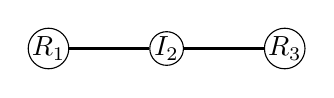
\begin{tikzpicture}[scale=1.5]
    % Draw a 7,11 network
    % First we draw the vertices
    \foreach \pos/\name in {{(1,0)/R_1}, {(2,0)/I_2}, {(3,0)/R_3}}
        \node[vertex] (\name) at \pos {$\name$};
    % Connect vertices with edges 
    \foreach \source/ \dest in {R_1/I_2, I_2/R_3}
        \path[edge] (\source) -- (\dest) ;
        
\end{tikzpicture}
%\end{minipage}
%}
\end{center}

\label{fig:strong_connectedness}
\caption{The state and the network in which the APEX equilibrium does not exist when $k=2$.}
\end{figure}

\begin{example}\label{ex_strong_connectedness}
Suppose that $k=2$ and $\theta=(R,I,R)$. The state and the network is represented in Figure ~\ref{fig:strong_connectedness}. Rebel 1 never learns $\theta_3$ since Inert 2 cannot reveal information about $\theta_3$. The APEX equilibrium does not exist in this scenario.
\end{example}

The following condition that works on the prior \textit{full support on strong connectedness} excludes the possibility of non-existence of APEX equilibrium. To this end, I begin with the definition of \textit{strong connectedness}.

\begin{definition}[Strong connectedness]
Given $G$, a state $\theta$ has strong connectedness if, for every two Rebels, there is a path consisting of Rebels to connect them.

\end{definition}  

In the language of graph theory, this definition is equivalent to: given $G$, $\theta$ has strong connectedness if the induced graph by $[R](\theta)$ is connected.

\begin{definition}[Full support on strong connectedness]
Given $G$, $\pi$ has full support on strong connectedness if 
\[\pi(\theta)>0\Leftrightarrow \text{ $\theta$ has strong connectedness }\] 
\end{definition}  

As a remark, the definition of the full support on strong connectedness is stronger than common knowledge about that every state has strong connectedness. This marginal requirement is subtle and is more convenient in constructing equilibrium.\footnote{The main result only requires a weaker version: $\pi(\theta)>0\Rightarrow \text{ $\theta$ has strong connectedness }$. However, working on this weaker version is at the expense of much tedious proof. Throughout this paper, I will stick to the original definition.} 

I am ready to state the main characterization of this paper:
\begin{theorem}[APEX equilibrium for the case of $1<k<n$]
\label{thm_main_result}
For any $n$-person repeated $k$-Threshold game with parameter $1<k<n$ played in networks, if networks are acyclic and if $\pi$ has full support on strong connectedness, then there is a $\delta^{*}$ such that an APEX equilibrium exists whenever $\delta>\delta^{*}$.\footnote{A network is acyclic if the path from $i$ to $j$ for all $i\neq j$ is unique.}

\end{theorem}

Constructing an APEX equilibrium, in this case, is more convoluted than that in the case of $k=n$. I illustrate the proof idea throughout this paper till Section, while leaving the formal proof in Appendix. Moreover, since the case of $k=2$ is trivial, the depictions throughout this paper below are all for $2<k<n$ cases. 

In the case of $k=n$, $T^{\theta}$ can be determined independently from $\theta$ by setting $T^{\theta}=n$, but it is not obvious how to obtain $T^{\theta}$ before an equilibrium has been constructed.\footnote{Readers might refer to the proof of Theorem \ref{thm_minor_thm}.} 
Moreover, the free-rider problem might exist in the current case (as demonstrated in Introduction), but this problem never occurs in the proposed APEX equilibrium for Theorem \ref{thm_minor_thm}. As for the punishment scheme, playing \textbf{stay} forever is not effective anymore since a deviation might only be seen by parts of players (network monitoring), and thus group punishment is hard to be executed.

after $t$. Share information. two digits.

Before we delve further into the logic of the proof of Theorem 2, I would like to introduce a game in Section \ref{sec:writing}: \textit{$T$-round writing game}. This is a simpler auxiliary scenario that mimics relevant features in the original game. In the $T$-round writing game, I allow players to write to each other. They will be endowed a writing technology so that they can write without cost (cheap talk) or with a cost function before they take actions. The readers who can also skip Section \ref{sec:writing} and Section \ref{sec:indem_writing} without confusion.
 
%The equilibrium construction of $T$-round writing game will be studied by means of examples and intentionally serve to demonstrate how to solve the free-rider problem. I then argue the equilibrium construction in the original game to be an analogue to the one in the $T$-round writing game. 

Roughly speaking, in the $T$-round writing game, players can write to share information about $\theta$ for $T$ rounds. They then play a one-shot $k$-threshold game at round $T+1$. Note that in an APEX equilibrium path in the original game, players would stop updating their belief after some finite time and keep playing the same action in the $k$-threshold game. The game form of the $T$-round writing game mimics the structure of the APEX equilibrium path in the original game. In Section \ref{sec:indem_writing}, I then further modify the $T$-round writing game to allow $T$ to be endogenously determined in the equilibrium, which is seamlessly analogous to the original game.\footnote{TBA.}  

  

\subsection{Deterministic $T$-round writing game}
\label{sec:writing}
The network, the set of states, and the set of players follow exactly the same definitions defined in Section \ref{sec:model}. In the deterministic $T$-round writing game, each player endows a \textit{writing technology}. A writing technology for player $i$ is a pair of $(W,M_i)$, in which $W=\{{\textbf{r}},\textbf{s}\}^L$, $L\in \mathbb{N}$, and $M\equiv \times_{i\in N}\times^T_{t=1}M^{t}_i$ recursively defined by
\[M^1_i=\{f|f:\Theta_{G_i}\rightarrow W\}\cup \{\emptyset\}\]
\[ \text{ for } 2\leq t \leq T\text{ , }M^{t}_i=\{f|f:\times_{j\in G_i}M^{t-1}_j\rightarrow W\}\cup \{\emptyset\}. \]
$W$ is interpreted as the set of sentence composed by letters \textbf{r} or \textbf{s} with length $L$, while $M_i$ can be understood as $i$'s grammar. The $\emptyset$ is interpreted as remaining silent. The meaning of ``$i$ writes to his neighbors at round $t$'' is equivalent to ``$i$ selects an $f\in M^t_i$ to get an element $w\in W$ according to $f$.  Moreover, $m$ can be observed by all $i$'s neighbors''. A sentence being a mixture of two sentences $w,w^{'}\in W$ is denoted as $w\oplus w^{'}$ with the property that $(w\oplus w^{'})_l=\textbf{r}$ if and only if $w_l=\textbf{r}$ or $w^{'}_l=\textbf{r}$ for all $l\in \{1,...,L\}$. 

The time line for the deterministic $T$-round writing game is as follows.
%\begin{enumerate}
%\item Nature chooses $\theta$ according to $\pi$.
%\item $\theta$ is then fixed throughout rounds.
%\item At $t=1,...,T$ round, players write to their neighbors. 
%\item At $T+1$ round, players play a one-shot $k$-Threshold game.
%\item The game ends.
%\end{enumerate}
\begin{table}[!htbp]
\begin{center}
\begin{tabular}{ll }
1.  & Nature chooses $\theta$ according to $\pi$. \\
2. & $\theta$ is then fixed throughout rounds.\\
3. & At $t=1,...,T$ round, players write to their neighbors. \\
4. & At $T+1$ round, players play a one-shot $k$-Threshold game.\\
5. & The game ends.
\end{tabular}
\end{center}
\end{table}
There is no discounting. A Rebel's payoff is the summation of his stage payoff across stages, while an Inert's payoff is set to be $1$. The equilibrium concept is a weak sequential equilibrium. The definition of APEX strategy is adapted as the strategy that induces ex-post outcome in the $k$-threshold game at $T+1$ round, and the definition of APEX equilibrium is adapted accordingly. In the examples below, let us focus on the configuration represented in Figure~\ref{fig:T-round-6} and Figure~\ref{fig:T-round-5} with $n=8$ and $L=8$. 

\begin{figure}

\begin{center}
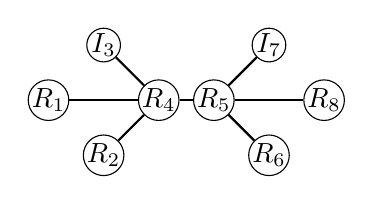
\begin{tikzpicture}[scale=0.7]
    % Draw a 7,11 network
    % First we draw the vertices
    \foreach \pos/\name in {{(1,2)/R_1}, {(2,1)/R_2}, {(5,1)/R_6}, {(6,2)/R_8}, {(3,2)/R_4}, {(4,2)/R_5}}
        \node[vertex] (\name) at \pos {$\name$};
    
    \foreach \pos/\name in {{(2,3)/I_3}, {(5,3)/I_7}}
    \node[unknown vertex] (\name) at \pos {$\name$};
    
%    \foreach \pos/\name in {{(3,2)/S_4}, {(4,2)/S_5}}
%    \node[selected vertex] (\name) at \pos {$\name$};
    
    % Connect vertices with edges 
    \foreach \source/ \dest in {R_1/R_4, R_2/R_4,I_3/R_4,R_4/R_5, R_5/R_6, R_5/I_7, R_5/R_8}
        \path[edge] (\source) -- (\dest) ;
        
\end{tikzpicture}
\end{center}
\caption{A configuration of the state and the network in which players 1,2,4,5,6,8 are Rebels while players 3,7 are Inerts.}
\label{fig:T-round-6}
\end{figure}

\begin{figure}

\begin{center}
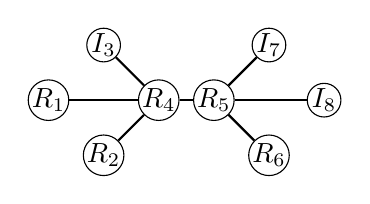
\begin{tikzpicture}[scale=0.7]
    % Draw a 7,11 network
    % First we draw the vertices
    \foreach \pos/\name in {{(1,2)/R_1}, {(2,1)/R_2}, {(5,1)/R_6}, {(3,2)/R_4}, {(4,2)/R_5}}
        \node[vertex] (\name) at \pos {$\name$};
    
    \foreach \pos/\name in {{(2,3)/I_3}, {(5,3)/I_7}, {(6,2)/I_8}}
    \node[unknown vertex] (\name) at \pos {$\name$};
    
%    \foreach \pos/\name in {{(3,2)/S_4}, {(4,2)/S_5}}
%    \node[selected vertex] (\name) at \pos {$\name$};
    
    % Connect vertices with edges 
    \foreach \source/ \dest in {R_1/R_4, R_2/R_4,I_3/R_4,R_4/R_5, R_5/R_6, R_5/I_7, R_5/I_8}
        \path[edge] (\source) -- (\dest) ;
        
\end{tikzpicture}
\end{center}
\caption{A configuration of the state and the network in which players 1,2,4,5,6 are Rebels while players 3,7,8 are Inerts.}
\label{fig:T-round-5}
\end{figure}

%
%\subsubsection{$T$-round writing game with cheap talk}
%\label{sec:cheap_talk}
\begin{example}[Deterministic $T$-round writing without cost---cheap talk]
\label{ex:cheap_talk}
Let $k=6$ ,$T=2$, and writing be costless. Consider the following strategy $\phi$. 

At $t=1$, $\phi$ specifies that the peripheral Rebels 1,2,6,8 remain silent. The central player Rebel 4 writes $(\textbf{r},\textbf{r},\textbf{s},\textbf{r},\textbf{r},\textbf{s},\textbf{s},\textbf{s})$. The central player Rebel 5 writes $(\textbf{s},\textbf{s},\textbf{s},\textbf{r},\textbf{r},\textbf{r},\textbf{s},\textbf{r})$ in the configuration in Figure \ref{fig:T-round-6} and writes $(\textbf{s},\textbf{s},\textbf{s},\textbf{r},\textbf{r},\textbf{r},\textbf{s},\textbf{s})$ in the configuration in Figure \ref{fig:T-round-5}.\footnote{The notion of ``peripheral'' and ``center'' will be formalized in Section \ref{sec:info}} On the path of $\phi$, Rebel 4's sentence thus reveals that players 1,2,4,5 are Rebels while player 3 is an Inert. It reveals so by the grammar: \textbf{r} is written in the $i$-th component if player $i$ is a Rebel while  \textbf{s} is written in the $j$-th component if player $j$ is Inert or unknown to Rebel 4. Rebel 5's sentence is written according to the same grammar. Note that the common knowledge of the network contributes to the ability in revealing the players' types. 

At $t=2$, $\phi$ specifies that the peripheral Rebels 1,2,6,8 still remain silent. Rebel 4 writes $(\textbf{r},\textbf{r},\textbf{s},\textbf{r},\textbf{r},\textbf{r},\textbf{s},\textbf{r})$ in the configuration in Figure \ref{fig:T-round-6} and writes $(\textbf{r},\textbf{r},\textbf{s},\textbf{r},\textbf{r},\textbf{r},\textbf{s},\textbf{s})$ in the configuration in Figure \ref{fig:T-round-5}. Rebel 5 writes exactly the same way as Rebel 4. This is to say Rebel 4 and 5 share information at $t=1$ and then coordinate to announce a mixture sentence at $t=2=T$. 

At $t=3=T+1$, all Rebels know whether or not the number of Rebels (by counting \textbf{r} in Rebel 4 or 5's combined sentence) is greater than or equal to $k=6$. This leads all Rebels to play the ex-post efficient outcome in the one-shot $k$-threshold game. 

%Suppose the configuration is that in Figure \ref{fig:T-round-5}. At $t=1$, similarly, $\phi$ specifies that Rebels 1,2,6,8 keep silent; Rebel 4 writes $(\textbf{r},\textbf{r},\textbf{s},\textbf{r},\textbf{r},\textbf{s},\textbf{s},\textbf{s})$; Rebel 5 writes $(\textbf{s},\textbf{s},\textbf{s},\textbf{r},\textbf{r},\textbf{r},\textbf{s},\textbf{s})$. At $t=2$, however, $\phi$ specifies that the peripheral Rebels 1,2,6,8 keep silent; Rebel 4 keeps silent; Rebel 5 keeps silent as well. On the path, keeping silent by Rebel 4 (or 5) reflects that Rebel 4 (or 5) knows that the total number of Rebels is less than $k=6$. At $t=3$, all Rebels know this relevant information and play the ex-post efficient outcome \textbf{stay}.

Let $\omicron$ be the belief system and the in-path belief be induced by $\phi$. The out-of-path strategy of $\phi$ specifies that, if a detectable deviation is made, then the Rebels who detect that deviation will remain silent until $t=T$ and then play \textbf{stay} at $t=T+1$.\footnote{A deviation could be, for instance, a wrong sentence that is not grammatical, is deviating from the in-path $\phi$, ..., etc} 
The out-of-path belief of $\omicron$ is to believe that all players who are not neighbors are all Inerts, which rationalizes the out-of-path strategy. Since writing is costless, and any deviation by Rebel 4 or 5 would strictly decrease the possibility of achieving an ex-post efficient outcome, the assessment $(\phi,\omicron)$ constitutes an APEX equilibrium.

\end{example}


%\begin{example}[Deterministic $T$-round writing with a fixed cost]
%\label{ex:fixed_cost_talk}
%Let $k=6$ and $T=2$. Suppose that writing incurs a fixed cost $\epsilon>0$ while keeping silent does not. Let us consider the assessment $(\phi,\omicron)$ in the above example. Since any deviation by Rebel 4 or 5 would strictly decrease the possibility to achieve the ex-post efficient outcome while the ex-post efficient outcome will give the maximum expected payoff for every Rebel at $t=3=T+1$ if the relevant information can be revealed then, if $\epsilon$ is sufficiently small, $(\phi,\omicron)$ also constitutes an APEX equilibrium.
%
%\end{example}


\begin{example}[Deterministic $T$-round writing with cost function and the free-rider problem]
\label{ex:cost_function_talk_fr}
Let $k=6$ and $T=2$. Suppose that remaining silent incurs no cost, but writing incurs a cost of  $\epsilon>0$ that is strictly decreasing with the number of \textbf{r} in a sentence. This is to say writing $(\textbf{r},\textbf{r},\textbf{r},\textbf{r},\textbf{r},\textbf{r},\textbf{r},\textbf{r})$ incurs the least cost while writing $(\textbf{s},\textbf{s},\textbf{s},\textbf{s},\textbf{s},\textbf{s},\textbf{s},\textbf{s})$ incurs the largest. 

If so, that assessment $(\phi, \omicron)$ in the previous example will no longer be an APEX equilibrium. To prove this, first note that the sentence of either Rebel 4 or 5's truthfully reveals their information at $t=1$ on the path of $\phi$. According to the above-mentioned, Rebel 4 will know the relevant information after $t=1$ (by common knowledge of the network) even if he deviates to writing that all his neighbors are Rebels.\footnote{This sentence is $(\textbf{r},\textbf{r},\textbf{r},\textbf{r},\textbf{r},\textbf{s},\textbf{s},\textbf{s})$, which incurs less cost than the truthfully reporting sentence $(\textbf{r},\textbf{r},\textbf{s},\textbf{r},\textbf{r},\textbf{s},\textbf{s},\textbf{s})$.}\footnote{If he remains silent, then this behavior will be considered as a deviation, and therefore he will never get the maximum payoff of $1$. Hence, he will avoid doing so.}
Rebel 5 is in the same situation as Rebel 4 and therefore will also write the sentence that indicates that all his neighbors are Rebels. However, these sentences are uninformative. It turns out that both of them will deviate, and neither of them can know the relevant information after $t=1$.
%\footnote{Actually, one can claim there is no APEX equilibrium in this case by contraposition. If there is one, say $(\phi^{'},\omicron^{'})$, then on the path of $\phi^{'}$, some Rebels should write and play differently in different configurations. Suppose Rebel 5 will play differently to truthfully reveal his information at $t=1$. Rebel 4 has two kinds of strategies then. He might write the least-cost sentence or he could write something depending on his information. For the former case, since Rebel 4 will be the only one who know the relevant information, he should write to Rebel 5 to let Rebel 5 pass this information to the remaining Rebels. However, it requires two rounds to pass it, but there is only one round left. For the latter case, if Rebel 4 truthfully reveal his information, the Rebel 5 will deviate to writing least-cost sentence; if Rebel 4's information is not truthfully reveal, there is a prior so that the ex-post outcome will not be played.}

Fortunately, the following example shows the free-rider problem can be solved. 
\end{example}



\begin{example}[Deterministic $T$-round writing with cost function and solving the free-rider problem]
\label{ex:cost_function_talk_solve_fr}
The free-rider problem that occurs in the previous example can be solved. The solution is to add more rounds to the game and exploit the assumption of common knowledge of the network. More precisely, let $k=6$ and $T=3$. 
%First note that if the previous strategy $\phi$ is extended to the current case so that Rebel 4 and 5 still simultaneously truthfully write their information at either $t=1$ or $t=2$, $\phi$ is not an equilibrium path by the same free-rider argument as the above. 

Consider a strategy $\dot{\phi}$ and focus on the interaction between Rebels 4 and 5. On the path of $\dot{\phi}$, at $t=1$, $\dot{\phi}$ specifies that the lowest-index Rebel between Rebels 4 and 5 is chosen to be a free rider, while the other one truthfully writes down his information. To be precise, at $t=2$, Rebel 4 will be the free rider---the person who writes the least-cost sentence; Rebel 5 writes $(\textbf{s},\textbf{s},\textbf{s},\textbf{r},\textbf{r},\textbf{r},\textbf{s},\textbf{r})$ in the configuration of Figure \ref{fig:T-round-6} while writing $(\textbf{s},\textbf{s},\textbf{s},\textbf{r},\textbf{r},\textbf{r},\textbf{s},\textbf{s})$ in the configuration of Figure \ref{fig:T-round-5}. 

At $t=2$, Rebel 5 remains silent. Rebel 4 writes the least-cost sentence if Rebel 5 writes $(\textbf{s},\textbf{s},\textbf{s},\textbf{r},\textbf{r},\textbf{r},\textbf{s},\textbf{r})$ at $t=1$ but remains silent if Rebel 5 writes $(\textbf{s},\textbf{s},\textbf{s},\textbf{r},\textbf{r},\textbf{r},\textbf{s},\textbf{s})$. Thus, the behavior of Rebel 4 at $t=2$ reveals the relevant information. 

At $t=3=T$, Rebel 4 remains silent. Rebel 5 writes the least-cost sentence if Rebel 4 writes the least-cost sentence at $t=2$ and remains silent if Rebel 4 remains silent then. 

It is straightforward to check that at $t=4=T+1$, all Rebels know the relevant information and play the ex-post efficient outcome accordingly. To construct an APEX equilibrium from $\dot{\phi}$, recall $(\phi,\omicron)$ and let the in-path belief of $\dot{\omicron}$ be induced by $\dot{\phi}$. The out-of-path strategy follows that in $\phi$, and the out-of-path belief follows that of $\omicron$.   

An observation is worthy to be noted: why is Rebel 5 willing to concede that Rebel 4 is chosen to be the free rider at $t=1$? The reason is as follows. He \textit{knows} that, by common knowledge of the network, he and Rebel 4 are in a free-rider problem. Moreover, again by common knowledge of the network, he knows that Rebel 4 knows this, Rebels 4 knows he knows that Rebel 4 knows this, ..., and so forth to infinite order of belief hierarchy. This is to say, at least in this case, Rebel 4 and 5 commonly know that they are engaged in a free-rider problem due to the common knowledge of the network. In Section \ref{sec:eq_rp}, this property of common knowledge about engaging in a free-rider problem will be formally characterized. This property is not merely a special case. It holds for any acyclic network in the constructed APEX equilibrium in the original game.  

\end{example}


\subsection{Indeterministic $T$-round writing game}
\label{sec:indem_writing}
In this section, the setting is exactly the same as that in the deterministic $T$-round writing game, except for that players will now jointly decide the round in which they will play the one-shot $k$-threshold game and then end the game. In other words, before they play the one-shot $k$-threshold game, they have to \textit{reach an agreement}---the common knowledge about which round is the terminal round ${T}$. 

The set of rounds is countably infinite and linearly ordered with generic element $t$. The writing technology is the same as that in deterministic $T$-round writing game, except for letting $W=\{\textbf{r},\textbf{s}\}^L\cup \{\textbf{r},\textbf{s}\}^{L^{'}}$ now. In the example below, let $L=8$ and $L^{'}=1$. 

Conceptually, there could be two kinds of rounds. In the first kind, players write to share information about $\theta$ (as they do in the deterministic $T$-round writing game). In the second kind, players write to form the common knowledge about ${T}$. Let us partition the set of rounds into two parts, $\Gamma$ and $\Gamma^{'}$, which represent the first kind and the second kind respectively. The round in $\Gamma$ is labelled $\gamma$ while the round in $\Gamma^{'}$ is labelled $\gamma^{'}_l$. The rounds are linearly ordered by $<$. To be more precise, the rounds are ordered as shown in Figure \ref{fig:ordered_writing}.
\begin{figure}

\label{fig:ordered_writing}
\[0^{'}_1<0^{'}_2<...<0^{'}_{l_0}<1<1^{'}_{1}<1^{'}_{2}<...<1^{'}_{l_1}<2<...,\]
where $l_0,l_1,...$ are all finite numbers.
\caption{The linearly ordered labelled rounds in the indeterministic $T$-round writing game.}
\end{figure}
An indeterministic $T$-round writing game is illustrated below. Along with it, an APEX equilibrium will be constructed. 

\begin{example}[Indeterministic $T$-round writing with cost function]
\label{ex:cost_function_talk_solve_fr_Indm}
Let $l_j=2$ for $j=0,1,...$. Suppose that the setting is exactly the same as that in Example \ref{ex:cost_function_talk_solve_fr}, except for that $T$ is not deterministic. Let us consider the path of a strategy $\psi$. At a round in $\Gamma^{'}$, $\psi$ specifies that, if a Rebel thinks ``it is certain that the total number of Rebels outnumbers $k$ and the nearest forthcoming round in $\Gamma$ is the terminal round,'' he will write $(\textbf{r})$. If a Rebel thinks ``it is possible but not certain that $\# [R](\theta)\geq k$,'' he will write $(\textbf{s})$. Otherwise, he will write $\emptyset$ to show that ``it is impossible that $\#[R](\theta)\geq k$ and the nearest forthcoming round in $\Gamma$ is the terminal round.'' 

According to this strategy, $t=1$ is not terminal if no Rebel has written $(\textbf{r})$ or $\emptyset$ before that. For instance, $t=1$ is not terminal in the configuration in Figure \ref{fig:T-round-6} and Figure \ref{fig:T-round-5}. 

If $t=1$ is not terminal, at $t=1$, Rebels 4 and 5 are in a free-rider problem as Example \ref{ex:cost_function_talk_fr} shows. $\psi$ solves it by specifying that Rebel 4 is the free rider and that Rebel 5 writes his information truthfully (as what $\dot{\phi}$ does in Example \ref{ex:cost_function_talk_solve_fr}). 

At $t=1^{'}_1$, Rebel 4 knows $\#[R](\theta)\geq k$ in the configuration in Figure \ref{fig:T-round-6} and knows $\#[R](\theta)< k$ in the configuration in Figure \ref{fig:T-round-5}. Therefore, he writes $(\textbf{r})$ and $\emptyset$ respectively for these two configurations. As for other Rebels, they write $(\textbf{s})$. 

After $t=1^{'}_1$, eventually, all Rebels will learn the relevant information (by seeing the writing of Rebel 4 at $t=1^{'}_1$) and terminate their writing at $t=2$. Therefore, $t=1$ is the terminal round, and the Rebels play a one-shot $k$-threshold game at $t=2$.

The strategy $\psi$ can be made to be an APEX equilibrium strategy in the same way as the previous examples. 


\end{example}


\subsection{Dispensability of writing technology}
\label{sec:dis_writing}
In essence, writing technology is dispensable, and repeated actions are sufficient to serve as a communication protocol to achieve an ex-post outcome in an equilibrium. In this section, I draw analogue between the writing game and the original game in Table \ref{table:analogue}. 

More precisely, in the equilibrium construction in the original game, let us partition the periods so that each part in the partition is analogous to a round in the writing game. The length of periods in a part is analogous to the length of a sentence. Since the actions played in a certain part of periods will incur an expected payoff, it is an analogue that writing is costly at a certain round in the writing game. The disjoint unions of period-sections also constitute a coarser partition of periods, which is analogous to partitioning the rounds. The analogue of $\Gamma$ is the set of \textit{periods for reporting} in the original game to emphasize that these periods are for reporting information about $\theta$. The analogue of $\Gamma^{'}$ is the set of \textit{periods for coordination} in the original game to emphasize that these periods are for coordinating to play the ex-post efficient outcome. The partition of periods is linearly ordered by $<$, and let us define a coarser partition with parts \textit{$t$-blocks} indexed by $t\in\{0,1,...\}$ along with the order of partition of periods as shown in Figure \ref{fig:ordered_original_game}. 

One could see that Figure \ref{fig:ordered_writing} and Figure \ref{fig:ordered_original_game} are seamlessly analogous to each other as Table \ref{table:analogue} shows.

\begin{figure}

\label{fig:ordered_original_game}
\[\underbrace{(\text{periods for coordination})}_{\text{$0$-block}}<\underbrace{(\text{periods for reporting})<(\text{periods for coordination})}_{\text{$1$-block}}<...\]
\caption{The linearly ordered period-sections in the repeated $k$-threshold game.}
\end{figure}


\begin{table}[!htbp]
\caption{The analogue between indeterministic $T$-round writing game and repeated $k$-threshold game}
\label{table:analogue}
\begin{center}
\begin{tabular}{ll }
Indeterministic $T$-round writing game & Repeated $k$-threshold game \\
\hline
\hline
A round & A range of periods\\
A sentence & A sequence of actions \\
The length of a sentence in a round & The length of a part of periods\\
A chosen digit in a sentence & A chosen action\\
The cost of writing a sentence & The expected payoff in a part of periods\\
The fixed grammar & The equilibrium path\\
\hline
\end{tabular}
\end{center}

\end{table}



Note that the notions of \textit{peripheral} and \textit{central} in Example \ref{ex:cheap_talk} is not yet formalized as well as analogized to the original game. I generalize these notions in the original game by defining \textit{information hierarchy} among players for each $t$-block below.


\subsubsection{Information hierarchy}
\label{sec:info}
The information hierarchy across Rebels in $G$ presents Rebels' information \textit{before entering the periods for reporting at $t$-block}. That is designated by a tuple \[(\{G^{t}_i\}_{i\in N}, \{I^{t}_i\}_{i\in N}, R^t,\theta).\]
$G^{t}_i$ represents \textit{the extended neighbors}: $j\in G^{t}_i$ if $j$ can be reached by $t$ consecutive edges from $i$, in which the endpoints of $t-1$ edges are both Rebels, while the remaining one consists of a Rebel and $i$ himself. $I^{t}_i$ represents \textit{the extended Rebel neighbors}: the set of Rebels in $G^t_i$. $R^t$ represents \textit{the active Rebels}: those Rebels who are \textit{active} in the sense that their extended Rebel neighbors are not a subset of their direct neighbors' extended Rebel neighbors. Those objects are defined by:

At $t=0$,
\[\text{if $\theta_i=I$, $G^{0}_i\equiv \emptyset$, $I^{0}_i\equiv \emptyset$.}\] 
\[\text{if $\theta_i=R$, $G^{0}_i\equiv \{i\}$, $I^{0}_i\equiv \{i\}$.}\] 
\[\text{$R^0\equiv [R](\theta)$.}\] 

At $t=1$,
\[\text{if $\theta_i=I$, $G^{1}_i\equiv \emptyset$, $I^{1}_i\equiv \emptyset$.}\] 
\[\text{if $\theta_i=R$, $G^{1}_i\equiv G_i$, $I^{0}_i\equiv G_i\cap R^0$.}\] 
\[\text{$R^1\equiv \{i\in R^0: \nexists j\in G_i \text{ such that }I^1_i\subseteq G^1_j\}$.}\] 

At $t>1$, 
\[\text{if $\theta_i=I$, $G^{t}_i\equiv \emptyset$, $I^{t}_i\equiv \emptyset$.}\] 
\[\text{if $\theta_i=R$, $G^{t}_i\equiv \bigcup_{j\in G_i} G^{t-1}_j$, $I^{t}_i\equiv \bigcup_{j\in G_i} I^{t-1}_j$, }\] 
\[\text{$I^{t}_{ij}\equiv I^{t-1}_i\cap I^{t-1}_j$ if $j\in G_i$.}\]
\[\text{$R^t\equiv \{i\in R^{t-1}: \nexists j\in G_i \text{ such that }I^t_i\subseteq G^t_j\}$.}\]



According to the definition above, the peripheral Rebels in the configuration of Figure \ref{fig:T-round-6} are active in $0$-block (in $R^0$) but not active in $1$-block (not in $R^1$), while the central players are active in both $0$-block and $1$-block. It can be shown that $R^t\subseteq R^{t-1}$ as follows. 
\begin{lemma}
\label{lemma_inclusion}
If the $\theta$ has strong connectedness, then 
\[R^t\subseteq R^{t-1}\] for all $t\geq 1$.
\end{lemma}

Is it sufficient to let only active Rebels share information about $\theta$ while $\theta$ can be revealed eventually? The answer is affirmative proven by Theorem \ref{lemma_empty} below, given that the network is acyclic and if the $\theta$ has strong connectedness.
\begin{theorem}
\label{lemma_empty}
If the network is acyclic and if the $\theta$ has strong connectedness, then 
\[[R](\theta)\neq \emptyset \Rightarrow \text{ there exists } t\geq 0 \text{ and } i\in R^t \text{ such that }I^{t+1}_i=[R](\theta).\] 
\end{theorem}


The strategy on the equilibrium path will specify how Rebels act according to the information hierarchy. $R^t$ will be those Rebels who are active in terms of sharing information in the periods for reporting in the $t$-block. 

%For convince, let us denote $I^{t+1}_{ij}=I^t_i\cap I^t_j$ if $j\in G_i\cap R^{t}$.  
\subsubsection{The equilibrium path in the periods for reporting}
\label{sec:eq_rp}
If there is no further mention, all the description in this section is for the APEX equilibrium path \textit{before} the terminal period $T^{\theta}$. For conciseness, let us shorten ``periods for reporting in $t$-block'' by $\Omicron^{t}$, denote $|\Omicron^t|$ as the length of $\Omicron^{t}$, and shorten \textbf{revolt} and \textbf{stay} to \textbf{r} and \textbf{s} receptively henceforth. 

$|\Omicron^{t}|$ is independent from $t$ and determines only the set of players. Firstly, assign each player $i$ a distinguishing prime number $x_i$ starting from $3$ (by exploiting the common knowledge of the network). Then let $|\Omicron^{t}|=x_1\otimes x_2\otimes...\otimes x_n$ , where $\otimes$ is the usual multiplication operator. The sequence of actions in $\Omicron^{t}$ is with length $|\Omicron^t|$ and would take one of the forms specified in the right column in Table \ref{Table_msg_form}. There, if $I\subseteq N$, then $x_{I}\equiv \otimes_{i\in I}x_i$. The abbreviations of these sequences are listed in the left column. Since these sequences in the periods for reporting are meant to share information about $\theta$, the terms ``playing the sequence'' and ``reporting the information'' are interchangeable and will be alternatively used.


\begin{table}[!htbp]
\caption{The notations for the sequences of actions in $\Omicron^t$ on the path}
\label{Table_msg_form}
\begin{center}
\begin{tabular}{l c c}
Notations && The sequences of actions\\
\hline
\hline
$\langle  I \rangle$ 				& $\equiv$ 			& $\langle \textbf{s},...,\textbf{s},\underbrace{\textbf{r},\textbf{s},...,\textbf{s}}_{x_{I}} \rangle$  \\
$\langle 1 \rangle$	 					& $\equiv$ 			& $\langle \textbf{s},...,\textbf{s},{\textbf{r}}\rangle$  \\
$\langle \textbf{all stay} \rangle$	 					& $\equiv$ 			& $\langle \textbf{s},...,\textbf{s},{\textbf{s}}\rangle$  \\
\hline
\end{tabular}
\end{center}
\end{table}


It is worth noting that this sequence constructed by prime numbers brings two benefits. Firstly, since the multiplication of distinguishing prime numbers can be uniquely factorized, the Rebels can utilize such sequence to precisely report players' identities. Secondly, the un-discounted expected payoff of playing $\langle I \rangle$ for some $I\subseteq N$ is always equal to $-1$, and therefore it is relatively easy to calculate. This is because, at any period in $\Omicron^{t}$, at most one player would play \textbf{r} by the property of prime number multiplication.\footnote{This statement holds given that there is no player who plays $\langle 1 \rangle$.} 

The sequence $\langle I \rangle$ is used for reporting $I\neq \emptyset$ when $I$ is a set of Rebels and sequence $\langle \textbf{all stay} \rangle$ is for the inactive Rebels to report nothing. The sequence $\langle 1 \rangle$ is intentionally crafted to tackle the free-rider problem. To see how $\langle 1 \rangle$ works, let us formally define the \textit{pivotal Rebel} and the \textit{free-rider problem}. 
\begin{definition}[Pivotal Rebels in $\Omicron^t$]
A Rebel $p$ is pivotal in $\Omicron^t$ if $p\in R^t$, $I^t_p\subset [R](\theta)$, $\# I^t_p<k$, and $p$ is certain that he will learn the relevant information in the end of $\Omicron^t$, given that each $i\in R^t$ reports $\langle I^t_i \rangle$.
\end{definition}

From the definition, a pivotal Rebel in $\Omicron^t$ is one who can learn the relevant information if all of his active Rebel neighbors truthfully report their information about $\theta$ to him. The pivotal Rebels can be further classified into two kinds: ones who can learn the true state, and ones who learn only the relevant information. When $k=6$, in the configuration in Figure \ref{fig:T-round-6}, only Rebels 4 and 5 are pivotal, and they are of the first kind; in the configuration in Figure \ref{fig:central_pivotal}, only Rebel 5 is pivotal, and he is of the first kind; in the configuration in Figure \ref{fig:k-1_pivotal}, only Rebel 4 pivotal, and he is of the second kind.

To be concise, let us call $p$ of the first kind by \textit{$\theta$-pivotal}. For the second kind, if the network is acyclic and if the prior has full support on strong connectedness, $p$ is the second kind in $\Omicron^{t}$ only if $I^{t}_p=k-1$. Since so, let us call the one with $I^t_p=k-1$ by \textit{$k-1$-pivotal}.\footnote{To show that a pivotal Rebel is the second kind in $\Omicron^{t}$ only if $I^{t}_p=k-1$, one can follow the same argument in Lemma \ref{lemma_inclusion} and Theorem \ref{lemma_empty}.}

\begin{figure}

\label{fig:central_pivotal}
\begin{center}
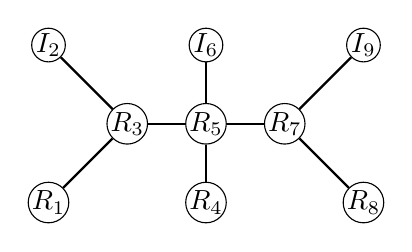
\begin{tikzpicture}[scale=1]
    % Draw a 7,11 network
    % First we draw the vertices
    \foreach \pos/\name in {{(1,1)/R_1}, {(1,3)/I_2}, {(2,2)/R_3}, {(3,1)/R_4}, {(3,2)/R_5}, {(3,3)/I_6}, {(4,2)/R_7}, {(5,1)/R_8}, {(5,3)/I_9}}
        \node[vertex] (\name) at \pos {$\name$};
    
    
    % Connect vertices with edges 
    \foreach \source/ \dest in {R_1/R_3, I_2/R_3, R_3/R_5, R_4/R_5, I_6/R_5, R_5/R_7, R_7/R_8, R_7/I_9}
        \path[edge] (\source) -- (\dest) ;
        
\end{tikzpicture}
\end{center}
\caption{A configuration of the state and the network in which player 1,3,5,4,7,8 are Rebels while players 2,4,9 are Inerts.}
\end{figure}

\begin{figure}

\label{fig:k-1_pivotal}
\begin{center}
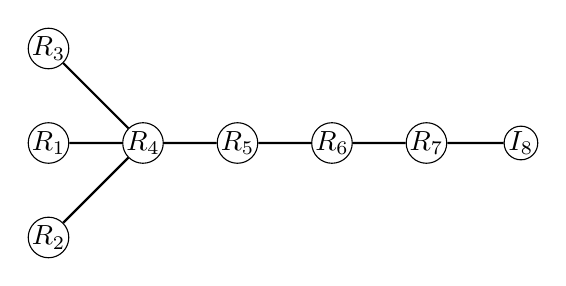
\begin{tikzpicture}[scale=1.2]
    % Draw a 7,11 network
    % First we draw the vertices
    \foreach \pos/\name in {{(2,2)/R_1}, {(2,1)/R_2}, {(2,3)/R_3}, {(3,2)/R_4}, {(4,2)/R_5}, {(5,2)/R_6}, {(6,2)/R_7}, {(7,2)/I_8}}
        \node[vertex] (\name) at \pos {$\name$};
    
    
    % Connect vertices with edges 
    \foreach \source/ \dest in {R_1/R_4, R_2/R_4,R_3/R_4,R_4/R_5, R_5/R_6, R_6/R_7, R_7/I_8}
        \path[edge] (\source) -- (\dest) ;
        
\end{tikzpicture}
\end{center}
\caption{A configuration of the state and the network in which player 1,2,3,4,5,6,7 are Rebels while player 8 is an Inert.}
\end{figure}

Below is the defined free-rider problem in $\Omicron^t$ .

\begin{definition}
A free-rider problem exists in $\Omicron^t$ if there are multiple $\theta$-pivotal Rebels in $\Omicron^t$.
\end{definition}



The following lemma is crucial. 
%it says that there will be at most two $\theta$-pivotal Rebels in $R^{t}$. Therefore, if there is a free-rider problem, it occurs between two $\theta$-pivotal Rebels. Moreover, if there are two of them, they are neighbors. (... it occurs between two Rebels who are neighbors.)
\begin{lemma}
\label{lemma_at_most_two_nodes}
If the network is acyclic and if $\pi$ has full support on strong connectedness, there are at most two $\theta$-pivotal Rebels in the $t$-block. Moreover, they are neighbors.\footnote{As a remark, Lemma \ref{lemma_at_most_two_nodes} is not true when the network is cyclic. To see this, consider a 4-player circle when $\theta=(R,R,R,R)$.}
\end{lemma}

Notably,

\begin{lemma}
\label{lemman_pivotals_CK}
If the network is acyclic and if $\pi$ has full support on strong connectedness, when there are two $\theta$-pivotal Rebels $p,p^{'}$ in the $t$-block, then they commonly know that they are $\theta$-pivotal Rebels at the beginning of $t$-block.
\end{lemma}

By Lemma ~\ref{lemman_pivotals_CK}, $\theta$-pivotal Rebels in $\Omicron^t$ can identify themselves at the beginning of $\Omicron^t$. It is essential, because if the free-rider problem occurs in $\Omicron^t$, the strategy can specify that the lowest indexed $\theta$-pivotal Rebel $p$ in the free-rider problem will play $\langle 1 \rangle$, while the other one $p^{'}$ will play $\langle I^t_{p^{'}} \rangle$ beforehand. In short, this knowledge is encoded in the belief system of an APEX equilibrium.

The assumption of acyclic network in Lemma \ref{lemman_pivotals_CK} is indispensable. In Section \ref{sec:cyclic}, there is a configuration in a cycle where there is no common knowledge of the free-rider problem if players still follow the equilibrium path working for Theorem \ref{thm_main_result}. 

Overall, the sequences played in $\Omicron^t$ on the path are listed in Table \ref{Table_msg_RP_path}.

\begin{table}[!htbp]
\caption{The sequences of actions played in $\Omicron^t$ on the path}
\label{Table_msg_RP_path}
\begin{center}
\begin{tabular}{l c}
Rebel $i$ & $i$ plays\\
\hline
\hline
$i\notin R^t$				& $\langle \textbf{all stay} \rangle$  \\
$i\in R^t$ but $i$ is not pivotal	 					 			& $\langle I^t_i \rangle$  \\
$i$ is $k-1$-pivotal	 					 			& $\langle 1 \rangle$  \\
$i$ is $\theta$-pivotal but not in the free-rider problem	 					 			& $\langle 1 \rangle$  \\
$i$ is in the free-rider problem with the lowest index	 					 			& $\langle 1 \rangle$  \\
$i$ is in the free-rider problem without the lowest index	 					 			& $\langle I^t_i \rangle$  \\
\hline
\end{tabular}
\end{center}
\end{table}


\subsubsection{The equilibrium path in the periods for coordination}
\label{sec:eq_cd}
In this section, I discuss the sequences of actions in the periods for coordination on the path. The term ``periods for coordination in $t$-block'' is shorten by $\Kappa^{t}$. If there is no further mention, all the description in this section is for the APEX equilibrium path \textit{before} the terminal period $T^{\theta}$. 

The main feature in the periods of coordination is that, whenever a Rebel $i$ is considered inactive starting at some $t$-block (i.e.~$i\notin R^t$ for some $t\in \mathbb{N}$), there is no strategy for $i$ to convince all Rebels that $\#[R](\theta)\geq k$ even though $i$ knows it and wants to propagandize it. The structure in the periods of coordination is much intrigued, and the periods are further partitioned by \textit{divisions} and \textit{sub-blocks}. I depict that below, where $(\Kappa)$ represents a certain range of periods for coordination. 



In $\Kappa^0$, 
\[\overbrace{\underbrace{( \Kappa) }_{\text{one sub-block}}}^{\text{$1$-division}} \overbrace{\underbrace{(\Kappa) }_{\text{one sub-block}}}^{\text{$2$-division}} \overbrace{\underbrace{(\Kappa) \cdot \cdot \cdot (\Kappa)}_{\text{$n$ sub-blocks}}}^{\text{$3$-division}}\] 

In $\Kappa^t$, $t>0$,
\[\overbrace{\underbrace{(\Kappa) \cdot \cdot \cdot (\Kappa)}_{\text{$n$ sub-blocks}}}^{\text{$1$-division}} \overbrace{\underbrace{(\Kappa) \cdot \cdot \cdot (\Kappa)}_{\text{$t+1$ sub-blocks}} }^{\text{$2$-division}} \overbrace{\underbrace{(\Kappa) \cdot \cdot \cdot (\Kappa)}_{\text{$n$ sub-blocks}}}^{\text{$3$-division}}\] 



%As in the equilibrium construction in Example \ref{ex:cost_function_talk_solve_fr_Indm}, the behavior in $CD^t$ is dependent on the behavior in $RP^t$ (when $t\geq 1$).

In the $t$-block, denote $\Kappa^t_{u,v}$ as the $v$-th sub-block in $u$-division and denote $|\Kappa^t_{u,v} |$ as the length of $\Kappa^t_{u,v}$. Similarly, denote $\Kappa^t_{u}$ as the $u$-division and denote $|\Kappa^t_{u} |$ as the length of $\Kappa^t_{u}$. Let us shorten \textbf{revolt} and \textbf{stay} to \textbf{r} and \textbf{s} receptively henceforth. On the path, the length of $|\Kappa^t_{u,v}|$ is determined. For all $v\in \{1,...,n\}$ let $|\Kappa^t_{u,v}|=n$ for $u=1,2$ and $|\Kappa^t_{u,v}|=1$ for $u=3$. The notations for the sequences of actions on the path are shown in Table ~\ref{Table_msg_coordination} shows.\footnote{Because, in the $3$-division, the length of the sequence of actions is 1, i.e.~playing an action, I dispense notations in the $3$-division for conciseness.}
For a Rebel $i$ on the equilibrium path, either $\langle i \rangle$ or $\langle \textbf{all stay} \rangle$ is seen. $\langle i \rangle$ is constructed for the purpose of simplifying calculation of expected payoff: there is at most one \textbf{r} played in $\Kappa^t_u$ for $t\geq 0$ and $u=1,2$.    

\begin{table}[!htbp]
\caption{The notations for the sequences of actions in $\Kappa^t_{u}$ for $u=1,2$, on the path}
\label{Table_msg_coordination}
\begin{center}
\begin{tabular}{l c c}
Notations & &The sequences of actions \\
\hline
\hline
$\langle i \rangle$ 				& $\equiv$ 			& $\langle \textbf{s},...,\textbf{s},\underbrace{\textbf{r},\textbf{s},...,\textbf{s}}_{i} \rangle$  \\
$\langle \textbf{all stay} \rangle$	 					& $\equiv$ 			& $\langle \textbf{s},...,\textbf{s},{\textbf{s}}\rangle$  \\
\hline
\end{tabular}
\end{center}
\end{table}


\paragraph{The equilibrium behavior on the path in $\Kappa^0$}
Since the $0$-block has a simpler structure, I begin with depicting the equilibrium path in $\Kappa^0$, which is shown in Table \ref{Table_cd0}. There, I describe the information of Rebel $i$ by whether $i$ has learnt the relevant information. It is not standard but more intuitive, while the full description can be found in Appendix. Notice that if Rebel $i$ is certain that $\#[R](\theta)<k$, it must be the case that all Rebels are $i$'s neighbors by the full support on strong connectedness. All Rebels will also be certain about that immediately after $\Kappa^0_{1}$. Figure \ref{fig:central_less_k} illustrates this scenario when $3\leq k <n$, in which Rebel 5 is certain $\#[R](\theta)<k$ in $\Kappa^0_1$. Rebel 4 is certain of that immediately after $\Kappa^0_1$. The idea in Table \ref{Table_cd0} is as follows. $\Kappa^0_1$ is the periods for a Rebel to advocate the knowledge of $\# [R](\theta)<k$. A Rebel $i$ will initiate coordination to \textbf{s} by playing $\langle \textbf{all stay} \rangle$ if he knows $\# [R](\theta)<k$; otherwise, he will play $\langle i \rangle$. $\Kappa^0_2$ is the periods for a Rebel to advocate the knowledge of $\# [R](\theta)\geq k$. Rebel $i$ will initiate coordination to \textbf{r} by playing $\langle \textbf{all stay} \rangle$ if he knows $\# [R](\theta)\geq k$ and has player $\langle i \rangle$ in the previous division $\Kappa^0_1$; otherwise, he will play $\langle i \rangle$. $\Kappa^t_3$ is used for coordinating to play \textbf{r} or \textbf{s} contagiously.

\begin{figure}

\label{fig:central_less_k}
\begin{center}
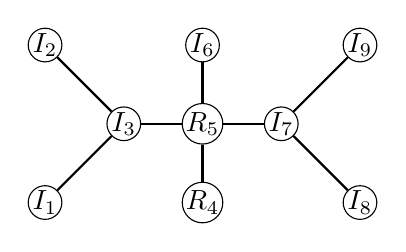
\begin{tikzpicture}[scale=1]
    % Draw a 7,11 network
    % First we draw the vertices
    \foreach \pos/\name in {{(1,1)/I_1}, {(1,3)/I_2}, {(2,2)/I_3}, {(3,1)/R_4}, {(3,2)/R_5}, {(3,3)/I_6}, {(4,2)/I_7}, {(5,1)/I_8}, {(5,3)/I_9}}
        \node[vertex] (\name) at \pos {$\name$};
    
    
    % Connect vertices with edges 
    \foreach \source/ \dest in {I_1/I_3, I_2/I_3, I_3/R_5, R_4/R_5, I_6/R_5, R_5/I_7, I_7/I_8, I_7/I_9}
        \path[edge] (\source) -- (\dest) ;
        
\end{tikzpicture}
\end{center}
\caption{A configuration of the state and the network in which player 4, 5 are Rebels while players 1,2,3,6,7,8,9 are Inerts.}
\end{figure}

The intriguing part might be ``how Rebel $i$ initiates the common knowledge about $\#[R](\theta)\geq k$.'' $i$ does so by \textit{first play $\langle i \rangle$ in $\Kappa^0_{1}$ and then play} $\langle \textbf{all stay} \rangle$ \textit{in $\Kappa^0_{2}$}. His behavior is then distinguishable from Rebels of other kinds. His neighbors will know $\#[R](\theta)\geq k$ immediately after $\Kappa^0_{2}$, and then all Rebels will know that by playing \textbf{r} contagiously in $\Kappa^0_{3}$. 

$i$ will not deviate to play $\langle \textbf{all stay} \rangle$ even though it might be undetectable. This is by the assumption of acyclic network. If $i$ does so, $i$ will be considered as an inactive Rebel afterwards by all of his neighbors. From this point on, he cannot update the belief held by his neighbors whose information hierarchy rank is no less than the one he pretends to be. More precisely, if he is a $R^{\dot{t}}$ Rebel but he pretends not to be one, he cannot influence the belief updating of the Rebels who are in $R^{t-1}$, $t\geq \dot{t}$.\footnote{This argument is due to Lemma \ref{lemma_inclusion} and the belief updating on the path described in Table \ref{Table_blf_up_cd01}, Table \ref{Table_blf_up_cd02}, Table \ref{Table_blf_up_rpt}, Table \ref{Table_blf_up_cdt1}, and Table \ref{Table_blf_up_cdt2}.} 
He then faces a positive probability that not enough Rebels can be informed of $\#[R](\theta)\geq k$. If this event happens, he will only get zero payoff. However, he can surely get the maximum payoff of $1$ afterwards and forever after $\Kappa^0_2$. Sufficiently high discount factor will deter this deviation. In essence, one major part of proof for Theorem \ref{thm_main_result} (in the appendix) follows the same argument.

%\begin{table}[!htbp]
%\caption{The sequences of actions played in $\Kappa^0_{1}$ on the path}
%\label{Table_cd011}
%\begin{center}
%\begin{tabular}{l c}
%Rebel $i$ 	 	&  	$i$ plays		 \\
%\hline
%\hline
%$i$ is certain $\#[R](\theta)<k$ 	& 	$\langle \textbf{all stay} \rangle$	\\
%$i\notin R^{1}$ and is uncertain $\#[R](\theta)\geq k$	& 	$\langle \textbf{all stay} \rangle$	\\
%$i\in R^{1}$ and is uncertain $\#[R](\theta)\geq k$ &  $\langle i \rangle$  \\
%$i$ is certain $\#[R](\theta)\geq k$ &  $\langle i \rangle$  \\
%\hline
%\end{tabular}
%\end{center}
%\end{table}


\begin{table}[!htbp]
\caption{The sequences of actions played in $\Kappa^0$ on the path}
\label{Table_cd0}
\begin{center}
\begin{tabular}{l c}
\multicolumn{2}{c}{The sequences of actions played in $\Kappa^0_{1}$ on the path}\\
Rebel $i$ 	 	&  	$i$ plays		 \\
\hline
\hline
$i$ is certain $\#[R](\theta)<k$ 	& 	$\langle \textbf{all stay} \rangle$	\\
$i\notin R^{1}$ and is uncertain $\#[R](\theta)\geq k$	& 	$\langle \textbf{all stay} \rangle$	\\
$i\in R^{1}$ and is uncertain $\#[R](\theta)\geq k$ &  $\langle i \rangle$  \\
$i$ is certain $\#[R](\theta)\geq k$ &  $\langle i \rangle$  \\
\hline
\\
\multicolumn{2}{c}{The sequences of actions played in $\Kappa^0_{2}$ on the path}\\
Rebel $i$ 	 	&  	$i$ plays		 \\
\hline
\hline
$i$ is certain $\#[R](\theta)<k$ 	& 	$\langle \textbf{all stay} \rangle$	\\
$i\notin R^{1}$ and is uncertain $\#[R](\theta)\geq k$	& 	$\langle \textbf{all stay} \rangle$	\\
$i\in R^{1}$ and is uncertain $\#[R](\theta)\geq k$ &  $\langle i \rangle$  \\
$i$ is certain $\#[R](\theta)\geq k$ &  $\langle \textbf{all stay} \rangle$  \\
\hline
\\
\multicolumn{2}{c}{The sequences of actions played in $\Kappa^0_{3}$ on the path}\\
Rebel $i$ 	 	&  	$i$ plays		 \\
\hline
\hline
$i$ is certain $\#[R](\theta)<k$ 	& 	$\langle \textbf{s} \rangle$	\\
$i\notin R^{1}$ and is uncertain $\#[R](\theta)\geq k$	& 	$\langle \textbf{s} \rangle$	\\
$i\in R^{1}$ and is uncertain $\#[R](\theta)\geq k$ &  $\langle \textbf{s} \rangle$  \\
$i$ is certain $\#[R](\theta)\geq k$ &  $\langle \textbf{r} \rangle$  \\
\hline
\end{tabular}
\end{center}
\end{table}

%\begin{table}[!htbp]
%\caption{The sequences of actions played in $\Kappa^0_{3}$ on the path}
%\label{Table_cd03v}
%\begin{center}
%\begin{tabular}{l c}
%Rebel $i$ 	 	&  	$i$ plays		 \\
%\hline
%\hline
%$i$ is certain $\#[R](\theta)<k$ 	& 	$\langle \textbf{s} \rangle$	\\
%$i\notin R^{1}$ and is uncertain $\#[R](\theta)\geq k$	& 	$\langle \textbf{s} \rangle$	\\
%$i\in R^{1}$ and is uncertain $\#[R](\theta)\geq k$ &  $\langle \textbf{s} \rangle$  \\
%$i$ is certain $\#[R](\theta)\geq k$ &  $\langle \textbf{r} \rangle$  \\
%\hline
%\end{tabular}
%\end{center}
%\end{table}
\clearpage

How Rebels update their belief that is being consistent with the equilibrium path after $\Kappa^0_1$ and $\Kappa^0_2$ is listed in Table \ref{Table_blf_up_cd01} and Table \ref{Table_blf_up_cd02}. One can track the evolution of information filtrations through Table \ref{Table_blf_up_cd01} to Table \ref{Table_blf_up_cd02}.

\begin{table}[!htbp]
\caption{The belief of $j\in G_i$ after observing $i$'s previous actions immediately after $\Kappa^0_{1}$}
\label{Table_blf_up_cd01}
\begin{center}
\begin{tabular}{l | c}
 	$i$ plays	  				  &  The event $j\in G_i$ assigns with probability one\\
\hline
\hline
In $\Kappa^0_{1}$	&				  \\
\hline
  $\langle \textbf{all stay} \rangle$	&    $i\notin R^1$ if $j\in R^1$ \\
  $\langle \textbf{all stay} \rangle$	&    $\#[Rebels](\theta)< k$ if $j\notin R^1$\\
  $\langle i \rangle$	&	  $i\in R^1$ or $\#[Rebels](\theta)\geq k$    \\
  \hline
\end{tabular}
\end{center}
\end{table}

\begin{table}[!htbp]
\caption{The belief of $j\in G_i$ after observing $i$'s previous actions immediately after $\Kappa^0_{2}$}
\label{Table_blf_up_cd02}
\begin{center}
\begin{tabular}{l  c | c}
 	$i$ plays	  	&  	  &The event $j\in G_i$ assigns with probability one \\
\hline
\hline
	In $\Kappa^0_{1}$		&			In $\Kappa^0_{2}$	&  \\
\hline
  $\langle \textbf{all stay} \rangle$	&  $\langle \textbf{all stay} \rangle$ &  $i\notin R^1$ if $j\in R^1$ \\
  $\langle \textbf{all stay} \rangle$	&  $\langle \textbf{all stay} \rangle$ &  $\#[Rebels](\theta)< k$ if $j\notin R^1$\\
  $\langle i \rangle$	&	$\langle \textbf{all stay} \rangle$ &  $\#[Rebels](\theta)\geq k$    \\
  $\langle i \rangle$	&	$\langle i \rangle$ &  $i\in R^1$  \\
  \hline
\end{tabular}
\end{center}
\end{table}

\clearpage

\paragraph{The equilibrium behavior on the path in $\Kappa^t$ for $t\geq 1$}
Next, I describe the equilibrium behavior on the path in $\Kappa^t$ whenever $t\geq 1$. Players' belief over states will now be contingent on the behavior in $\Omicron^t$ since Rebels share information in $\Omicron^t$. As an analogue to the grammar interpretation in the deterministic (or indeterministic) $T$-round writing game, I first illustrate how players update their belief after observing the equilibrium strategy on the path. After that, the in-path strategy contingent on players' belief is introduced. Players' information filtrations evolve from Table \ref{Table_blf_up_rpt} through Table \ref{Table_blf_up_cdt1} to Table \ref{Table_blf_up_cdt2}.

\begin{table}[!htbp]
\caption{The belief of $j\in G_i$ after observing $i$'s previous actions immediately after $\Omicron^t$ }
\label{Table_blf_up_rpt}
\begin{center}
\begin{tabular}{l | c}
 $i$ plays  		&	 The event $j\in G_i$ assigns with probability one \\
\hline
\hline
 In $\Omicron^t$		&					 \\
\hline
$\langle \textbf{all stay} \rangle$  &     $i\notin R^t$ and $I^{t+1}_{ji}=I^t_j$ \\
$\langle I^t_{i} \rangle$  &     $i\in R^t$ and $I^{t+1}_{ji}=I^t_j\cap I^t_{i}$ \\
$\langle 1 \rangle$  & 	  $i$ is pivotal    \\
  \hline
\end{tabular}
\end{center}
\end{table}



\begin{table}[!htbp]
\caption{The belief of $j\in G_i$ after observing $i$'s previous actions immediately after $\Kappa^t_1$ {contingent} on $\Omicron^t$ }
\label{Table_blf_up_cdt1}
\begin{center}
\begin{tabular}{l  l | c}
 $i$ plays	&			  & The event $j\in G_i$ assigns with probability one \\
\hline
\hline
	  In $\Omicron^t$	 	&		In $\Kappa^t_{1,1}$	&				  \\
\hline
$\langle \textbf{all stay} \rangle$  & $\langle i \rangle$	&    $i\notin R^t$ and $I^{t+1}_{ji}=I^t_j$  \\
$\langle I^t_{i} \rangle$  & $\langle \textbf{all stay} \rangle$	&    $\#[Rebels](\theta)< k$ \\
$\langle I^t_{i} \rangle$  & $\langle i \rangle$	&    $i\in R^t$ and $I^{t+1}_{ji}=I^t_j\cap I^t_{i}$,  or $\#[Rebels](\theta)\geq k$ \\
$\langle 1 \rangle$  & $\langle \textbf{all stay} \rangle$	&	  $\#[Rebels](\theta)< k$    \\
$\langle 1 \rangle$  & $\langle i \rangle$	&	  $\#[Rebels](\theta)\geq k$  \\
  \hline
\end{tabular}
\end{center}
\end{table}

\begin{table}[!htbp]
\caption{The belief of $j\in G_i$ after observing $i$'s previous actions immediately after $\Kappa^0_{2}$ {contingent} on $\Omicron^t$ and $\Kappa^0_{2}$ }
\label{Table_blf_up_cdt2}
\begin{center}
\begin{tabular}{l  l l | c}
 $i$ plays  	&		&  	  &The event $j\in G_i$ assigns with probability one\\
\hline
\hline
In $\Omicron^t$			&	In $\Kappa^t_{1,1}$			&			In $\Kappa^t_{2,1}$		&   \\
\hline
$\langle \textbf{all stay} \rangle$  & $\langle i \rangle$	&  $\langle \textbf{all stay} \rangle$ &  $i\notin R^t$ and $I^{t+1}_{ji}=I^t_j$  \\
$\langle I^t_{i} \rangle$  & $\langle \textbf{all stay} \rangle$	&  $\langle \textbf{all stay} \rangle$ &  $\#[Rebels](\theta)< k$ \\
$\langle I^t_{i} \rangle$  & $\langle i \rangle$	&  $\langle \textbf{all stay} \rangle$ &  $\#[Rebels](\theta)\geq k$ \\
$\langle I^t_{i} \rangle$  & $\langle i \rangle$	&  $\langle i \rangle$ &  $i\in R^t$ and $I^{t+1}_{ji}=I^t_j\cap I^t_{i}$ \\
$\langle 1 \rangle$  & $\langle \textbf{stay} \rangle$	&	$\langle \textbf{all stay} \rangle$ &  $\#[Rebels](\theta)< k$    \\
$\langle 1 \rangle$  & $\langle i \rangle$	&	$\langle \textbf{all stay} \rangle$ &  $\#[Rebels](\theta)\geq k$  \\
  \hline
\end{tabular}
\end{center}
\end{table}

\clearpage

The delicate part in $\Kappa^t$ is how a pivotal Rebel $p$ propagandizes the relevant information. $p$ does so by playing $\langle \textbf{all stay} \rangle$ in $\Kappa^{t}_{1,1}$ in the case of $\#[R](\theta)< k$, while playing $\langle p \rangle$ in the case of $\#[R](\theta)\geq k$. Notice that playing $\langle \textbf{all stay} \rangle$ in $\Kappa^{t}_{1,1}$ by $p$ will immediately inform $p$'s neighbors that $\#[R](\theta)< k$. On the contrary, playing sequence other than $\langle \textbf{all stay} \rangle$ has not yet revealed $\#[R](\theta)\geq k$ since that might be played by other non-pivotal Rebels. 

In $\Kappa^{t}_{2,1}$, however, $p$ reveals $\#[R](\theta)\geq k$ by playing $\langle \textbf{all stay} \rangle$, which is a costless sequence of actions. It might not seem intuitive at first sight, but it effectively prevents a potential free-rider problem: there are two pivotal Rebels, say $p$ and $p^{'}$, who have already known $\#[R](\theta)\geq k$ in $\Kappa^t$. If initiating the common knowledge about $\#[R](\theta)\geq k$ incurs negative payoff, $p$ or $p^{'}$ will have the incentive (again!) to let the other one initiate it. Playing $\langle \textbf{all stay} \rangle$ in $\Kappa^t_{2,1}$ proudly becomes the initiation sequence by its cheapness.

The remaining argument is why other non-pivotal Rebels, say $i$, do not mimic the pivotal Rebels' behavior to play $\langle 1 \rangle$ in $\Omicron^t$. If $i$ plays $\langle 1 \rangle$, all Rebels will learn the relevant information immediately after $\Kappa^t_2$ based on the belief updating on the path. It implies that the beginning of $t+1$-block is the terminal period. He will not learn the relevant information after that because the belief updating will be also terminated. However, he is still uncertain whether he can learn the relevant information in $\Omicron^t$ since he is not pivotal. Since that the ex-post efficient outcome gives him the maximum payoff at every $\theta$, and that he will learn the relevant information eventually on the equilibrium path, he prefers not to deviate given that the discount factor is high enough.\footnote{Since $R^t$ Rebels share information on the equilibrium path, by Theorem \ref{lemma_empty}, the belief updating in Table \ref{Table_blf_up_rpt}, Table \ref{Table_blf_up_cdt1}, and Table \ref{Table_blf_up_cdt2}, and the in-path behavior in Table \ref{Table_cdt}, the relevant information is learnt by every Rebel eventually on the path.} 
The proof of Theorem \ref{thm_main_result} heavily follows the arguments of this kind.

As a complement, I depict equilibrium strategy contingent on players' belief in Table \ref{Table_cdt}. The idea in Table \ref{Table_cdt} is as follows. $Kappa^t_1$ is the periods for a Rebel to advocate the knowledge of $\# [R](\theta)<k$. A Rebel $i$ will initiate coordination to \textbf{s} by playing $\langle \textbf{all stay} \rangle$ in $Kappa^t_{1,1}$ if he knows $\# [R](\theta)<k$; otherwise, he will play $\langle i \rangle$. $Kappa^t_2$ is the periods for a Rebel to advocate the knowledge of $\# [R](\theta)\geq k$. A Rebel $i$ will initiate coordination to \textbf{r} by playing $\langle \textbf{all stay} \rangle$ in $\Kappa^t_{2,1}$ if he knows $\# [R](\theta)\geq k$ and has player $\langle 1 \rangle$ in the previous periods $\Omicron^t$; otherwise, he will play $\langle i \rangle$. $K^t_3$ is used for coordinating to play \textbf{r} or \textbf{s} contagiously.

\begin{table}[!htbp]
\caption{The sequences of actions played in $\Kappa^t$, $t\geq 1$ on the path}
\label{Table_cdt}
\begin{center}
\begin{tabular}{l c}
\multicolumn{2}{c}{The sequences of actions played in $\Kappa^t_{1,v}$ for $t\geq 1$ and for $v=1,2,...,n$ on the path}\\
Rebel $i$ 	 	&  	$i$ plays		 \\
\hline
\hline
$i$ is certain $\#[R](\theta)<k$ 	& 	$\langle \textbf{all stay} \rangle$	\\
$i\notin R^{t}$ and is uncertain $\#[R](\theta)\geq k$	& 	$\langle i \rangle$	\\
$i\in R^{t}$ and is uncertain $\#[R](\theta)\geq k$ &  $\langle i \rangle$  \\
$i$ is certain $\#[R](\theta)\geq k$ &  $\langle i \rangle$  \\
\hline
\\
\multicolumn{2}{c}{The sequences of actions played in $\Kappa^t_{2,v}$ for $t\geq 1$ for $v=1$ on the path}\\
Rebel $i$ 	 	&  	$i$ plays		 \\
\hline
\hline
$i$ is certain that $\#[R](\theta)<k$ 	& 	$\langle \textbf{all stay} \rangle$	\\
$i\notin R^{t}$ and is uncertain $\#[R](\theta)\geq k$	& 	$\langle \textbf{all stay} \rangle$	\\
$i\in R^{t}$ and is uncertain $\#[R](\theta)\geq k$ &  $\langle i \rangle$  \\
$i$ is certain that $\#[R](\theta)\geq k$ &  $\langle \textbf{all stay} \rangle$  \\
\hline
\\
\multicolumn{2}{c}{The sequences of actions played in $\Kappa^t_{2,v}$ for $t\geq 1$ for $v=2,...,t+1$ on the path}\\
Rebel $i$ 	 	&  	$i$ plays		 \\
\hline
\hline
$i$ is certain that $\#[R](\theta)<k$ 	& 	$\langle \textbf{all stay} \rangle$	\\
$i\notin R^{t}$ and is uncertain $\#[R](\theta)\geq k$	& 	$\langle \textbf{all stay} \rangle$	\\
$i\in R^{t}$ and is uncertain $\#[R](\theta)\geq k$ &  $\langle \textbf{all stay} \rangle$  \\
$i$ is certain that $\#[R](\theta)\geq k$ &  $\langle i \rangle$  \\
\hline
\\
\multicolumn{2}{c}{The sequences of actions played in $\Kappa^t_{3}$ for $t\geq 1$ on the path}\\
Rebel $i$ 	 	&  	$i$ plays		 \\
\hline
\hline
$i$ is certain that $\#[R](\theta)<k$ 	& 	$\textbf{s}$	\\
$i\notin R^{1}$ and is uncertain $\#[R](\theta)\geq k$	& 	$ \textbf{s} $	\\
$i\in R^{1}$ and is uncertain $\#[R](\theta)\geq k$ &  $ \textbf{s} $  \\
$i$ is certain that $\#[R](\theta)\geq k$ &  $ \textbf{r} $  \\
\hline
\end{tabular}
\end{center}
\end{table}


%\begin{table}[!htbp]
%\caption{The sequences of actions played in $\Kappa^t_{2,v}$ for $t\geq 1$ for $v=1$ on the path}
%\label{Table_cdt21}
%\begin{center}
%\begin{tabular}{l c}
%Rebel $i$ 	 	&  	$i$ plays		 \\
%\hline
%\hline
%$i$ is certain that $\#[R](\theta)<k$ 	& 	$\langle \textbf{all stay} \rangle$	\\
%$i\notin R^{t}$ and is uncertain $\#[R](\theta)\geq k$	& 	$\langle \textbf{all stay} \rangle$	\\
%$i\in R^{t}$ and is uncertain $\#[R](\theta)\geq k$ &  $\langle i \rangle$  \\
%$i$ is certain that $\#[R](\theta)\geq k$ &  $\langle \textbf{all stay} \rangle$  \\
%\hline
%\end{tabular}
%\end{center}
%\end{table}


%\begin{table}[!htbp]
%\caption{The sequences of actions played in $\Kappa^t_{2,v}$ for $t\geq 1$ for $v=2,...,t+1$ on the path}
%\label{Table_cdt2t}
%\begin{center}
%\begin{tabular}{l c}
%Rebel $i$ 	 	&  	$i$ plays		 \\
%\hline
%\hline
%$i$ is certain that $\#[R](\theta)<k$ 	& 	$\langle \textbf{all stay} \rangle$	\\
%$i\notin R^{t}$ and is uncertain $\#[R](\theta)\geq k$	& 	$\langle \textbf{all stay} \rangle$	\\
%$i\in R^{t}$ and is uncertain $\#[R](\theta)\geq k$ &  $\langle \textbf{all stay} \rangle$  \\
%$i$ is certain that $\#[R](\theta)\geq k$ &  $\langle i \rangle$  \\
%\hline
%\end{tabular}
%\end{center}
%\end{table}


%\begin{table}[!htbp]
%\caption{The sequences of actions played in $\Kappa^t_{3}$ for $t\geq 1$ on the path}
%\label{Table_cdt3v}
%\begin{center}
%\begin{tabular}{l c}
%Rebel $i$ 	 	&  	$i$ plays		 \\
%\hline
%\hline
%$i$ is certain that $\#[R](\theta)<k$ 	& 	$\textbf{s}$	\\
%$i\notin R^{1}$ and is uncertain $\#[R](\theta)\geq k$	& 	$ \textbf{s} $	\\
%$i\in R^{1}$ and is uncertain $\#[R](\theta)\geq k$ &  $ \textbf{s} $  \\
%$i$ is certain that $\#[R](\theta)\geq k$ &  $ \textbf{r} $  \\
%\hline
%\end{tabular}
%\end{center}
%\end{table}
\clearpage






\subsubsection{Out-of-path belief and learning on the path}
In this section, I demonstrate examples to show the learning process on the equilibrium path and illustrate the out-of-path belief. Whenever Rebel $i$ detects a deviation at period $s$, he forms the following belief: 
\begin{equation}
\label{eq_grim_trigger}
\sum_{\theta \in \{\theta:\theta_j=I,j\notin G_i\}}\beta^{\pi,\tau}_{G_i}({\theta}|h^{\dot{s}}_{G_i})=1 \text{, for all $\dot{s}\geq s$}.
\end{equation}
Thus, if $\# I^0_i<k$, he will play \textbf{stay} forever after he detects a deviation. This out-of-path belief serves as a grim trigger. 

The example below demonstrates how players learn on the equilibrium path. Let us take the configuration in Figure \ref{fig:T-round-6}.\footnote{As Example \ref{ex:cost_function_talk_solve_fr_Indm} does.}
\begin{example}
Let $k=6$. Players have their prime numbers as $(x_1,x_2,...,x_8)=(3,5,7,11,13,17,19,23)$.

At $\Kappa^0_{1}$, Rebels 1, 2, 6, and 8 play $\langle \textbf{all stay} \rangle$; Rebels 4 and 5 play $\langle 4 \rangle$ and $\langle 5 \rangle$ respectively. 

At $\Kappa^0_{2}$, Rebels 1, 2, 6, and 8 play $\langle \textbf{all stay} \rangle$; Rebels 4 and 5 play $\langle 4 \rangle$ and $\langle 5 \rangle$ respectively.

At $\Kappa^0_{3,v}$, for $v=1,..,n$, all Rebels play $\textbf{s} $. 

Immediately after $\Kappa^0_{3}$, all Rebels are uncertain about $\# [R](\theta)\geq k$.

At $\Omicron^1$, $|\Omicron^1|=111546435$. Rebels 1, 2, 6, and 8 play 
\[\langle \textbf{all stay} \rangle=\langle \overbrace{\textbf{s},...,\textbf{s}}^{111546435} \rangle.\] Rebel 4 plays 
\[\langle 1 \rangle=\langle \overbrace{\textbf{s},...,\textbf{s},\textbf{r}}^{111546435} \rangle.\] Rebel 5 plays 
\[\langle \{4,5,6,8\} \rangle=\langle \overbrace{\textbf{s},...,\textbf{s},\underbrace{\textbf{r},\textbf{s},...,\textbf{s}}_{55913}}^{111546435} \rangle.\] Immediately after $\Omicron^1$, Rebel 4 is certain $\# [R](\theta)\geq k$ while Rebels 1,2,5,6,8 are not.

At $\Kappa^1_{1,v}$ for $v=1,...,n$, Rebel $i$ plays $\langle i \rangle$. Rebels 1,2,4,5 are certain $\# [R](\theta)\geq k$, while the others are not.

At $\Kappa^1_{2,1}$, Rebels 6 and 8 play $\langle 6 \rangle$ and $\langle 8 \rangle$ respectively. Rebels 1,2,4,5 play $\langle \textbf{all stay} \rangle$. Immediately after $\Kappa^1_{2,1}$, Rebels 6 and 8 also know $\# [R](\theta)\geq k$.

At $\Kappa^1_{2,2}$, all Rebels play $\langle \textbf{all stay} \rangle$.

At $\Kappa^1_{2,v}$ for $v=1,...,n$, all Rebels play $\textbf{r}$. 

After $\Kappa^1_{2,n}$, all Rebels play \textbf{r} forever. 



\end{example}






\section{Discussion}
\label{sec:varies}
%
%


%\subsubsection{Variation: Rebels with different levels of efforts}
%
%We may also consider a model in which players contribute different levels of efforts to a collective action. Let the set of states of nature be $\hat{\Theta}=\Theta \times \Xi$, where $\Theta=\{Rebel,Inert\}^n$ and $\Xi=\{1,2,...,k\}^n$. Let $\hat{\theta}=(\theta,e)$ be a state of nature. After $\hat{\theta}$ is realized, a player $i$ will hold an endowment $e_i$, where $e_i\in \{1,2,...,k\}$. The payoff structure is modified as the following.
%\begin{enumerate}
%\item $u_{Rebel_i}(a_{Rebel_i},a_{-\theta_i})=b_i$ if $a_{Rebel_i}=\textbf{revolt}$ and $\sum_{j:a_{\theta_j}=\textbf{revolt}}e_j\geq k$
%\item $u_{Rebel_i}(a_{Rebel_i},a_{-\theta_i})=-e_i$ if $a_{Rebel_i}=\textbf{revolt}$ and $\sum_{j:a_{\theta_j}=\textbf{revolt}}e_j< k$
%\item $u_{Rebel_i}(a_{Rebel_i},a_{-\theta_i})=0$ if $a_{Rebel_i}=\textbf{stay}$
%\item $u_{Inert_i}(a_{Inert_i},a_{-\theta_i})=1$ if $a_{Inert_i}=\textbf{stay}$
%\end{enumerate}
%
%
%
%After $\hat{\theta}$ is realized, players repeatedly play the above game in a network $G$. To see that the strategies constructed in previous section is still an equilibrium, we can transform $(G,\hat{\Theta})$ to $(G^{'},\hat{\Theta}^{'})$, where each player $i$ is attached with $\#e_i$ different players in $G^{'}$, and $\hat{\Theta}^{'}=\Theta\times \{1\}^{n}$. 
%
%
\subsection{Cyclic networks}
\label{sec:cyclic}


Scenarios in cyclic networks substantially differ from the acyclic counterpart. The free-rider problem becomes intractable in cyclic networks, at least in the way of my equilibrium construction. Let us consider the configuration in Figure \ref{fig:cyclic_network}.

\begin{figure}[!h]

\label{fig:cyclic_network}
\begin{center}
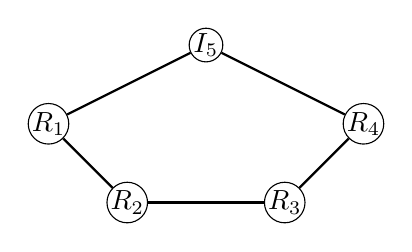
\begin{tikzpicture}[scale=1]
    % Draw a 7,11 network
    % First we draw the vertices
    \foreach \pos/\name in {{(2,3)/R_1}, {(3,2)/R_2}, {(5,2)/R_3}, {(6,3)/R_4}, {(4,4)/I_5}}
        \node[vertex] (\name) at \pos {$\name$};
    
    
    % Connect vertices with edges 
    \foreach \source/ \dest in { R_1/R_2, R_2/R_3, R_3/R_4, R_4/I_5, I_5/R_1}
        \path[edge] (\source) -- (\dest) ;
        
\end{tikzpicture}
\end{center}
\caption{A configuration of the state and the network in which player 1,2,3,4 are Rebels while player 5 is an Inert.}
\end{figure}

Suppose $k=4$ and the period $s$ at the beginning of $1$-block is not terminal. By the definition of pivotal Rebel in Section \ref{sec:eq_rp}, Rebel 2 and 3 are $\theta$-pivotal. From the perspective of Rebel 2's view, the type of player 5 could be Inert. Therefore, Rebel 2 does not know whether or not Rebel 1 is pivotal. Similarly, Rebel 2 does not know whether or not Rebel 3 is pivotal, \textit{even though} player 3 is indeed $\theta$-pivotal. Therefore there is no common knowledge of the free-rider problem at period $s$.  

However, suppose we cut the edge between player 4 and 5, Rebel 2 knows that he is the only $\theta$-pivotal Rebel.


%I leave a conjecture in this paper and end this section.
%
%\begin{conjecture}
%For any $n$-person repeated $k$-Threshold game with parameter $ k < n$ played in any network,
%if $\pi$ has full support on strong connectedness, then there exists a $\delta^{*}$ such that an APEX equilibrium exists whenever $\delta>\delta^{*}$.
%\end{conjecture}
%
%
%

\subsection{Payoff as signals}
The hidden payoff assumption can be relaxed without changing the main result. One may consider a situation in which the static payoff not only depends on players' joint efforts but also on a random shock, say the weather. To fix the idea, there is a public signal $y\in \{r,s\}$ generated by Rebels' actions. Let Rebel $i$'s payoff function be $u_{R}(a_{R},y)$ and $u_{R}(\textbf{stay},r)=u_{R}(\textbf{stay},s)=u_0$. The distribution of $y_1$ and $y_2$ is 
\begin{eqnarray*}
p_{rr} &=& \mathrm {Pr}(y=r|\#\{j:a_j\textbf{revolt}\}\geq k) \\
p_{rs}=1-p_{rr} &=& \mathrm {Pr}(y=r|\#\{j:a_j\textbf{revolt}\}< k) \\
p_{ss} &=& \mathrm {Pr}(y=s|\#\{j:a_j\textbf{revolt}\}< k) \\
p_{sr}=1-p_{ss} &=& \mathrm {Pr}(y=s|\#\{j:a_j\textbf{revolt}\}\geq k) \\
\end{eqnarray*}
such that
\begin{equation*}
p_{rr}u_{R}(\textbf{revolt}, r)+p_{sr}u_{R}(\textbf{revolt}, s)>u_0>p_{rr}u_{R}(\textbf{revolt}, r)+p_{ss}u_{R}(\textbf{revolt}, s).
\end{equation*}
and
\begin{equation*}
1>p_{rs}>0,1>p_{ss}>0.
\end{equation*}

The APEX equilibrium constructed for Theorem \ref{thm_main_result} (in Section \ref{sec:dis_writing} and in Appendix) is still a one in this scenario. Note that in that APEX equilibrium path, at most one \textbf{revolt} can occur at every period before some Rebel plays $\langle 1 \rangle$. This implies that the signal $y$ is completely uninformative before some Rebel plays $\langle 1 \rangle$. If a Rebel $i$ deviates to play $\langle 1 \rangle$ in $\Omicron^t$ at some $t$ to get information from $y$, he will not learn the relevant information after $\Omicron^t$ since the terminal period will immediately come after $t$-block. He will however learn the relevant information and play the ex-post efficient outcome if he keeps himself on the path.

If $p_{rr}$ or $p_{ss}=1$, then construct an APEX equilibrium as follows: all Rebels play \textbf{revolt} in the first period and then keep playing \textbf{revolt} or \textbf{stay} contingent on the signals $y=r$ or $y=s$ respectively.


\section{Conclusion}
\label{sec:con}
I model a coordination game and illustrate the learning processes generated by strategies in a (weak) sequential equilibrium to answer the question proposed in the beginning: what kind of networks can conduct coordination in a collective action with information barrier. In the equilibrium, players transmit the relevant information by encoding such information by their actions as time goes by. Since there might be an negative expected payoff in coding information, the potential free-rider problems might occur to impede the learning process. My result show that if the network is acyclic, players can always learn the underlying relevant information and conduct the coordination only by actions. In cyclic networks, however, what kinds of equilibrium strategies can lead to learning the relevant information still remains to be answered.


The construction of the communication protocol by actions exploits the assumption of the common knowledge of the network and the finite type space. Since the relevant information has been parametrized as a threshold in the stage game, players can acquire this information by jointly incrementally reporting their own private information period by period. The major punishment to deter deviation is then the joint shifting to play that same action as the stopping to update information. The threshold game thus seems a potential model in proofing that a communication protocol by actions not only leads a learning process but also constitutes an equilibrium to reveal the relevant information in finite time.

Existing literatures in political science and sociology have recognized the importance of social network in influencing individual's behavior in participating social movements ( \citep{Passy2003}\citep{McAdam2003}\citep{Siegel2009}). This paper views networks as routes for communication in which rational individuals initially have local information but they can influence nearby individuals by taking actions. Such influence may take long time to travel across individuals and the whole process incurs inefficient outcomes in many periods. A characterization in the speed of information transmission across a network is not answered here, although it is an important topic in investigating the most efficient way to let the information be spread. This question would remain for the future research.



\bibliographystyle{abbrvnat}	% (uses file "plain.bst")
\bibliography{bigref}		% expects file "myrefs.bib"


\appendix
\section{Appendix}
\subsection{The APEX equilibrium for Theorem \ref{thm_main_result}}
\subsubsection{Equilibrium path}
By definition of information hierarchy, 
\begin{eqnarray*}
G^t_i & = & \bigcup_{k_1\in G_i}\bigcup_{k_2\in G_{k_0}}...\bigcup_{k_{t}\in G_{k_{t-1}}}G_{k_{t}}\\
&= & \{j\in N: \text{$\exists$ a path $(i,k_1...k_{l},j)$ s.t.~$l\leq t-1$ and $\theta_i=\theta_{k_1}=...=\theta_{k_l}=R$}\}.
\end{eqnarray*}
Let us further define
\begin{definition}[Extended tree by $G^t_i$]
\label{def:ext_tree}
\begin{eqnarray*}
X^t_i & \equiv &  \{j\in N: \\
	& & \text{$\exists$ a path $(i,k_1...k_{l},j_1,...,j_m,j)$ s.t.~$l\leq t-1$ and $\theta_i=\theta_{k_1}=...=\theta_{k_l}=\theta_{j_1}=R$}\}.\\
\end{eqnarray*}
\end{definition}
$X^t_i $ represents the tree extended by $G^t_i$. By assuming the network is acyclic, this is equivalent to the set of all possible Rebels in $G$. 

The equilibrium will be represented as a \textit{finite register machine}. 
\begin{definition}[Finite register machine]
A finite register machine for $i$ consists of finite registers $\Sigma$. A register is a tuple \[(\Omega, \times_{G_i}A_R,f,\lambda),\] in which $\Omega$ are sets of events induced by $H_i$. $\times_{G_i}A_R$ is the sets of input. $f:\Omega\rightarrow A_{R}$ assigns an action to each event. $\lambda: \Omega\times Y \rightarrow \Sigma$ is the transition function. There is a set of initial registers. 
\end{definition}

Note that $i$'s register specifies $i$'s action according his information at a certain period, but does not characterize $i$'s information. The definition of a register machine here is more like the \textit{switch function}. The information of $i$ up to period $s$ has been characterized as $P_i(\theta)\times \{h^s_{G_i}\}\times H^s_{N\setminus G_i}$ as that in Section \ref{sec:model}. 

\begin{definition}[$m$-register in $t$-block]
A $m$-register in a (sub)block or a division is the register in the $m$-th period in that (sub)block or division.
\end{definition}

To shorten the notation, denote $m\dashv\Gamma$ as the $m$-register in the (sub)block or division $\Gamma$.

\begin{definition}[Terminal register]
A register is terminal if its every $f\in F$ is a constant and the image of $\lambda \in \Lambda$ is a singleton containing itself. 
\end{definition}

Though players act as if acting a whole sequence, they in fact act period by period. For convenience, for any finite sequence of action $\langle \rangle$, denote $\langle \rangle_m$ as the $m$-th (counting from the beginning) component in $\langle \rangle$, and denote $\langle \rangle(m)$ as the prefix of $\langle \rangle$ with length $m$. Let us also shorten action \textbf{revolt} to be \textbf{r} and \textbf{stay} to be \textbf{s}. 
\clearpage
\noindent{\textbf{Equilibrium path in $\Kappa^0$}}

\begin{landscape}
\begin{table}[!htbp]
\caption{The $m\dashv\Kappa^0_{1}$ on the path}
\begin{center}
\begin{tabular}{c c | c | c | c }
\multicolumn{5}{c}{$1\leq m \leq |\Kappa^0_1|-1$}\\
$\omega_i$ 	 & 	   &	$f(\omega_i)$  &	$a_{G_i}$ & $\lambda(\omega_i,y)$ \\
\hline
\hline

$\# X^t_i<k$  	& 	 &$\langle \textbf{all stay} \rangle_m$ &	& terminal \textbf{s}\\
$i\notin R^1$, $\# X^t_i\geq k$, $I^1_i< k$  	&  &$\langle \textbf{all stay} \rangle_m$ & 	& $m+1\dashv\Kappa^0_{1}$\\
$i\in R^1$, $\# X^t_i\geq k$, $I^1_i< k$  	& 	 &$\langle i \rangle_m$	&  & $m+1\dashv \Kappa^0_{1}$\\
$i\in R^1$, $\# X^t_i\geq k$, $I^1_i\geq k$  	& 	 &$\langle i \rangle_m$	&  & $m+1\dashv \Kappa^0_{1}$\\
\hline
\multicolumn{5}{c}{$m=|\Kappa^0_1|$}\\
$\omega_i$ 	 & 	   &	$f(\omega_i)$  &	$a_{G_i}$ & $\lambda(\omega_i,y)$ \\
\hline
\hline
$\# X^t_i<k$  	& 	& $\langle \textbf{all stay} \rangle_m$	&     & terminal \textbf{s}\\
$i\notin R^1$, $\# X^t_i\geq k$, $I^1_i< k$   	& all $j$ play $\langle \textbf{all stay} \rangle(m-1)$ & $\langle \textbf{all stay} \rangle_m$	 & all $j$ play \textbf{s} & terminal \textbf{s}\\
$i\notin R^1$, $\# X^t_i\geq k$, $I^1_i< k$   	& $\exists j$ plays $\langle j \rangle(m-1)$ & $\langle \textbf{all stay} \rangle_m$	& such $j$ plays $\langle j \rangle_m$  & $1\dashv \Kappa^0_2$\\
$i\in R^1$, $\# X^t_i\geq k$, $I^1_i< k$   	& 	& $\langle i \rangle_m$	&& $1\dashv \Kappa^0_2$ \\
$i\in R^1$, $\# X^t_i\geq k$, $I^1_i\geq k$  	& 	& $\langle i \rangle_m$ &	& $1\dashv \Kappa^0_2$ \\
\hline
\end{tabular}
\end{center}
\end{table}



\end{landscape}

\begin{landscape}
\begin{table}[!htbp]
\caption{The $m\dashv\Kappa^0_{2}$ on the path, where $1\leq m \leq |\Kappa^0_2|-1$}
\begin{center}
\begin{tabular}{c c | c | c | c}
\multicolumn{5}{c}{$1\leq m < |\Kappa^0_1|$}\\
$\omega_i$ 	 & 	   &	$f(\omega_i)$  &	$a_{G_i}$ & $\lambda(\omega_i,y)$ \\
\hline
\hline
$i\notin R^1$  	& & $\langle \textbf{all stay} \rangle_m$	&    & $m+1\dashv \Kappa^0_{2}$\\
$i\in R^1$, $I^1_i< k$  	& $\exists j$, $j$ plays $<j>_j=s$	& $\langle \textbf{all stay} \rangle_m$	& 	& $m+1\dashv \Kappa^0_{2}$\\
$i\in R^1$, $I^1_i< k$  	& $\forall j$, $j$ plays $<j>_j=r$ 	& $\langle i \rangle_m$	& 	& $m+1\dashv \Kappa^0_{2}$\\
$i\in R^1$, $I^1_i\geq k$  	& 	& $\langle \textbf{all stay} \rangle_m$	&	& $m+1\dashv \Kappa^0_{2}$\\
\hline
\multicolumn{5}{c}{$m= |\Kappa^0_1|$}\\
$\omega_i$ 	 & 	   &	$f(\omega_i)$  &	$a_{G_i}$ & $\lambda(\omega_i,y)$ \\
\hline
\hline
$i\notin R^1$  	& $\forall j$ play $\langle j \rangle(m-1)$    & $\langle \textbf{all stay} \rangle_m$	& $\forall j$ play $\langle j \rangle_m$	& $1\dashv \Kappa^0_{3}$\\
$i\notin R^1$  	& $\exists j$ plays $\langle \textbf{all stay} \rangle(m-1)$   & $\langle \textbf{all stay} \rangle_m$	& such $j$ plays $\langle \textbf{all stay} \rangle_m$	& terminal \textbf{r}\\
$i\in R^1$, $I^1_i< k$   	& $\forall j$ play $\langle j \rangle(m-1)$ 	& $\langle i \rangle_m$	&  $\forall j$ play $\langle j \rangle_m$	& $1\dashv \Kappa^0_{3}$ \\
$i\in R^1$, $I^1_i< k$   	&  $\exists j$ plays $\langle \textbf{all stay} \rangle(m-1)$ 	& $\langle i \rangle_m$	& such $j$ plays $\langle \textbf{all stay} \rangle_m$	&  terminal \textbf{r}\\
$i\in R^t$, $I^1_i\geq k$  	& 	& $\langle \textbf{all stay} \rangle_m$	& 	& terminal \textbf{r} \\
\hline
\end{tabular}
\end{center}
\end{table}

\end{landscape}






\clearpage

\begin{table}[!htbp]
\caption{The $m\dashv\Kappa^0_{3}$ on the path, where $1\leq m \leq |\Kappa^0_3|-1$}
\begin{center}
\begin{tabular}{c c | c | c | c}
\multicolumn{5}{c}{$1\leq m < |\Kappa^0_1|$}\\
$\omega_i$ 	 & 	   &	$f(\omega_i)$  &	$a_{G_i}$ & $\lambda(\omega_i,y)$ \\
\hline
\hline
  	&	& \textbf{s} & $\forall j$ play $\textbf{s}$ 	& $m+1\dashv \Kappa^0_{3}$\\
  	&  & \textbf{s}  &  $\exists j$ play $\textbf{r}$  	& terminal \textbf{r}\\
\hline
\multicolumn{5}{c}{$1\leq m = |\Kappa^0_1|$}\\
$\omega_i$ 	 & 	   &	$f(\omega_i)$  &	$a_{G_i}$ & $\lambda(\omega_i,y)$ \\
\hline
\hline
  	& 	& \textbf{s} & $\forall j$ play $\textbf{s}$ 	& $1\dashv \Omicron^1$\\
  	&  & \textbf{s}  &  $\exists j$ play $\textbf{r}$  	& terminal \textbf{r}\\
\hline
\end{tabular}
\end{center}
\end{table}





\clearpage

\noindent \textbf{Equilibrium path in $\Omicron^t$}
Let $m_j=|\Omicron^t|-x_{I^t_j}$ be the period in which $j$ report $I^t_j$ (i.e.~the period where \textbf{r} occurs in $\langle I^t_j \rangle$). Define $I^{t+1}_i(m)\equiv I^t_i\cup(\bigcup_{j\in G_i, m_j<m}I^t_j)$ to be the information of $i$ up to the $m$-th period in $\Omicron^t$. Similarly, define $i$'s extended neighbors to be $G^{t+1}_i(m)\equiv G^t_i\cup(\bigcup_{j\in G_i, m_j<m}I^t_j)$. Then define $X^{t+1}_i(m)$ to be the extended tree from $G^t_i(m)$ in the same way as Definition \ref{def:ext_tree}.


\begin{landscape}
\begin{table}[!htbp]
\caption{The $m\dashv\Omicron^t$ on the path, where $1\leq m<|\Omicron^t|$}
\begin{center}
\begin{tabular}{c c | c | c | c}
\multicolumn{5}{c}{$1\leq m < |\Kappa^0_1|$}\\
$\omega_i$ 	 & 	   &	$f(\omega_i)$  &	$a_{G_i}$ & $\lambda(\omega_i,y)$ \\
\hline
\hline
$i\notin R^t$  	& 								& $\langle \textbf{all stay} \rangle_m$		&  			& $m+1\dashv \Omicron^t$ \\
$i\in R^t$, not free rider, not $k-1$-pivotal	  	& $I^{t+1}_i(m-1)<k$, $X^{t+1}_i(m)\geq k$		    & $\langle I^t_i \rangle_m$ 		&    			& $m+1\dashv \Omicron^t$ \\
$i\in R^t$, not free rider, not $k-1$-pivotal		 	&  $I^{t+1}_i(m-1)< k$, $X^{t+1}_i(m-1)<k$			&  $\langle \textbf{all stay} \rangle_m$	& 									  & terminal \textbf{s} \\
$i\in R^t$, not free rider, not $k-1$-pivotal	 	&  $I^{t+1}_i(m-1)\geq k-1$			& $\langle 1 \rangle_m$ 	& 									  & $m+1\dashv \Omicron^t$ \\
$i\in R^t$, the free rider  	&  $X^{t+1}_i(m-1)\geq k$ & $\langle 1 \rangle_m$ 		& 				  & $m+1\dashv \Omicron^t$ \\
$i\in R^t$, the free rider  	&  		$X^{t+1}_i(m-1)<k$					&  $\langle \textbf{all stay} \rangle_m$		& 										  & terminal \textbf{s} \\
$i\in R^t$, $i$ is $k-1$-pivotal  	&  $X^{t+1}_i(m-1)\geq k$ & $\langle 1 \rangle_m$ 	& 											 & $m+1\dashv \Omicron^t$ \\
$i\in R^t$, $i$ is $k-1$-pivotal  	&  	$X^{t+1}_i(m-1)<k$		&  $\langle \textbf{all stay} \rangle_m$	& 											 & terminal \textbf{s} \\
\hline
\multicolumn{5}{c}{$1\leq m < |\Kappa^0_1|$}\\
$\omega_i$ 	 & 	   &	$f(\omega_i)$  &	$a_{G_i}$ & $\lambda(\omega_i,y)$ \\
\hline
\hline
%$X^{t+1}_i(m)<k$  	&                                    & 											&				 				& to terminal \textbf{s}\\
$i\notin R^t$  	& 								& $\langle \textbf{all stay} \rangle_m$		&  			& $1\dashv \Omicron^t$ \\
$i\in R^t$, not free rider, not $k-1$-pivotal	  	& $I^{t+1}_i(m-1)<k$, $X^{t+1}_i(m)\geq k$		    & $\langle I^t_i \rangle_m$ 		&    			& $1\dashv \Omicron^t$ \\
$i\in R^t$, not free rider, not $k-1$-pivotal		 	&  $I^{t+1}_i(m-1)< k$, $X^{t+1}_i(m-1)<k$			&  $\langle \textbf{all stay} \rangle_m$	& 									  & terminal \textbf{s} \\
$i\in R^t$, not free rider, not $k-1$-pivotal	 	&  $I^{t+1}_i(m-1)\geq k-1$			& $\langle 1 \rangle_m$ 	& 									  & $m+1\dashv \Omicron^t$ \\
$i\in R^t$, the free rider  	&  $X^{t+1}_i(m-1)\geq k$ & $\langle 1 \rangle_m$ 		& 				  & $m+1\dashv \Omicron^t$ \\
$i\in R^t$, the free rider  	&  		$X^{t+1}_i(m-1)<k$					&  $\langle \textbf{all stay} \rangle_m$		& 										  & terminal \textbf{s} \\
$i\in R^t$, $i$ is $k-1$-pivotal  	&  $X^{t+1}_i(m-1)\geq k$ & $\langle 1 \rangle_m$ 	& 											 & $m+1\dashv \Omicron^t$ \\
$i\in R^t$, $i$ is $k-1$-pivotal  	&  	$X^{t+1}_i(m-1)<k$		&  $\langle \textbf{all stay} \rangle_m$	& 											 & terminal \textbf{s} \\
\hline
\end{tabular}
\end{center}
\end{table}


\end{landscape}
\clearpage



\noindent \textbf{Equilibrium path in $\Kappa^t$ for $t\geq 1$}
\begin{table}[!htbp]
\caption{The $m\dashv\Kappa^t_{1,v}$ on the path, where $1\leq m<|\Kappa^t_{1,v}|$, $v=1,...,n$}
\begin{center}
\begin{tabular}{c c | c | c | c}
\multicolumn{5}{c}{$1\leq m < |\Kappa^0_1|$}\\
$\omega_i$ 	 & 	   &	$f(\omega_i)$  &	$a_{G_i}$ & $\lambda(\omega_i,y)$ \\
\hline
\hline
$X^{t+1}_i<k$  	&                                & $\langle \textbf{all stay} \rangle_m$		&				 				& to terminal \textbf{s}\\
$X^{t+1}_i\geq k$  	& 						& $\langle i \rangle_m$		&  $\exists j=m\text{ such that } a_j=\textbf{s}$	& terminal \textbf{s}\\
$X^{t+1}_i\geq k$ 	& 						& $\langle i \rangle_m$		&  $\forall j\text{ such that } a_j= \langle j \rangle_m$	& $m+1\dashv \Kappa^t_{1,v}$\\
\hline
\multicolumn{5}{c}{$1\leq m < |\Kappa^0_1|$}\\
$\omega_i$ 	 & 	   &	$f(\omega_i)$  &	$a_{G_i}$ & $\lambda(\omega_i,y)$ \\
\hline
\hline
$X^{t+1}_i<k$  	&                                & 											&				 				& to terminal \textbf{s}\\
$X^{t+1}_i\geq k$ & 						& $\langle i \rangle_m$		&  $\exists j=m\text{ such that } a_j=\textbf{s}$	& terminal \textbf{s}\\
$X^{t+1}_i\geq k$ 	& 						& $\langle i \rangle_m$		&  $\forall j\text{ such that } a_j= \langle j \rangle_m$	& $1\dashv \Kappa^t_{1,v+1}$\\
\hline
\multicolumn{5}{c}{$1\leq m < |\Kappa^0_1|$}\\
\hline
\hline
$X^{t+1}_i\geq k$ 	& 						& $\langle i \rangle_m$		&  $\exists j=m\text{ such that } a_j=\textbf{s}$	& terminal \textbf{s}\\
$X^{t+1}_i\geq k$ & 						& $\langle i \rangle_m$		&  $\forall j\text{ such that } a_j= \langle j \rangle_m$	& $1\dashv \Kappa^t_{2,1}$\\
\hline
\multicolumn{5}{c}{$1\leq m < |\Kappa^0_1|$}\\
$\omega_i$ 	 & 	   &	$f(\omega_i)$  &	$a_{G_i}$ & $\lambda(\omega_i,y)$ \\
\hline
\hline
$X^{t+1}_i\geq k$ 	& 						& $\langle i \rangle_m$		&  $\exists j=m\text{ such that } a_j=\textbf{s}$	& terminal \textbf{s}\\
$X^{t+1}_i\geq k$ 	& 						& $\langle i \rangle_m$		&  $\forall j\text{ such that } a_j= \langle j \rangle_m$	& $1\dashv \Kappa^t_{2,1}$\\
\hline
\end{tabular}
\end{center}
\end{table}


\clearpage



\begin{table}[!htbp]
\caption{The $m\dashv\Kappa^t_{2,v}$ on the path, where $1\leq m<|\Kappa^t_{2,v}|$, $v=1,...,t+1$}
\begin{center}
\begin{tabular}{c l | c | c | c}
\multicolumn{5}{c}{$1\leq m < |\Kappa^0_1|$}\\
$\omega_i$ 	 & 	   &	$f(\omega_i)$  &	$a_{G_i}$ & $\lambda(\omega_i,y)$ \\
\hline
\hline
$I^{t+1}_i< k$  	& 	$\exists j$, $\langle j \rangle_j=\textbf{s}$	& $\langle \textbf{all stay} \rangle_m$		&  	& $m+1\dashv \Kappa^t_{2,v}$\\
$I^{t+1}_i< k$  	& 	$\forall j$, $\langle j \rangle_j=\textbf{r}$	& $\langle i \rangle_m$		&  	& $m+1\dashv \Kappa^t_{2,v}$\\
$I^{t+1}_i\geq k$	 & 				& $\langle \textbf{all stay} \rangle_m$ 	& 		& $m+1\dashv \Kappa^t_{2,v}$\\
\hline
\multicolumn{5}{c}{$1\leq m < |\Kappa^0_1|$}\\
$\omega_i$ 	 & 	   &	$f(\omega_i)$  &	$a_{G_i}$ & $\lambda(\omega_i,y)$ \\
\hline
\hline
$I^{t+1}_i< k$  	& 	$\exists j$, $\langle j \rangle_j=\textbf{s}$	& $\langle \textbf{all stay} \rangle_m$		&  	& $m+1\dashv \Kappa^t_{2,v}$\\
$I^{t+1}_i< k$  	& 	$\forall j$, $\langle j \rangle_j=\textbf{r}$	& $\langle i \rangle_m$		&  	& $m+1\dashv \Kappa^t_{2,v}$\\
$I^{t+1}_i\geq k$	 & 				& $\langle \textbf{all stay} \rangle_m$ 	& 		& $m+1\dashv \Kappa^t_{2,v}$\\
\hline
\multicolumn{5}{c}{$1\leq m < |\Kappa^0_1|$}\\
$\omega_i$ 	 & 	   &	$f(\omega_i)$  &	$a_{G_i}$ & $\lambda(\omega_i,y)$ \\
\hline
\hline
$I^{t+1}_i< k$  	& 	$\exists j$, $\langle j \rangle_j=\textbf{s}$	& $\langle \textbf{all stay} \rangle_m$		&  	& $m+1\dashv \Kappa^t_{2,v}$\\
$I^{t+1}_i< k$  	& 	$\forall j$, $\langle j \rangle_j=\textbf{r}$	& $\langle i \rangle_m$		&  	& $m+1\dashv \Kappa^t_{2,v}$\\
$I^{t+1}_i\geq k$	 & 				& $\langle \textbf{all stay} \rangle_m$ 	& 		& $m+1\dashv \Kappa^t_{2,v}$\\
\hline
\multicolumn{5}{c}{$1\leq m < |\Kappa^0_1|$}\\
$\omega_i$ 	 & 	   &	$f(\omega_i)$  &	$a_{G_i}$ & $\lambda(\omega_i,y)$ \\
\hline
\hline
$I^{t+1}_i< k$  	& 	$\exists j$, $\langle j \rangle_j=\textbf{s}$	& $\langle \textbf{all stay} \rangle_m$		&  	& terminal \textbf{r}\\
$I^{t+1}_i< k$  	& 	$\forall j$, $\langle j \rangle_j=\textbf{r}$	& $\langle i \rangle_m$		&  	& $m+1\dashv \Kappa^t_{2,v}$\\
$I^{t+1}_i\geq k$	 & 				& $\langle \textbf{all stay} \rangle_m$ 	& 		& terminal \textbf{r}\\
\hline
\end{tabular}
\end{center}
\end{table}




\clearpage









\begin{table}[!htbp]
\caption{The $m\dashv\Kappa^t_{3}$ on the path, where $1\leq m \leq |\Kappa^t_3|-1$}
\begin{center}
\begin{tabular}{c c | c | c | c}
\multicolumn{5}{c}{$1\leq m < |\Kappa^0_1|$}\\
$\omega_i$ 	 & 	   &	$f(\omega_i)$  &	$a_{G_i}$ & $\lambda(\omega_i,y)$ \\
\hline
\hline
  	&	& \textbf{s} & $\forall j$ play $\textbf{s}$ 	& $m+1\dashv \Kappa^t_{3}$\\
  	&  & \textbf{s}  &  $\exists j$ play $\textbf{r}$  	& terminal \textbf{r}\\
\hline
\multicolumn{5}{c}{$1\leq m < |\Kappa^0_1|$}\\
$\omega_i$ 	 & 	   &	$f(\omega_i)$  &	$a_{G_i}$ & $\lambda(\omega_i,y)$ \\
\hline
\hline
 	& 	& \textbf{s} & $\forall j$ play $\textbf{s}$ 	& $1\dashv \Omicron^{t+1}$\\
  	&  & \textbf{s}  &  $\exists j$ play $\textbf{r}$  	& terminal \textbf{r}\\
\hline
\end{tabular}
\end{center}
\end{table}




\clearpage
\subsection{Missing proofs}
%\label{appx_network}
\noindent\textbf{Proof of Lemma ~\ref{lemma_learn}}
%\begin{lemma*}[Learning in the APEX equilibrum]
%If the assessment $(\tau^*,\mu^{*})$ is an APEX equilibrium, then for all $\theta\in \Theta$, there is a finite time $T^{\theta}_i$ for every Rebel $i$ such that $\sum_{\theta\in\{\theta:[R](\theta)\geq k\}}\beta^{\pi,\tau^*}_{G_i}(\theta|h^{s}_{G_i})=$ either $1$ or $0$
%whenever $s\geq T^{\theta}_i$.
%\end{lemma*}
\begin{proof}
The proof is done by contraposition. Suppose Rebels' strategies constitute an APEX equilibrium. By definition of the APEX equilibrium, at every $\theta$, there is a period $T^{\theta}$ when all Rebels' actions start to repeat themselves. Let $T=\max_{\theta\in \Theta}{T^{\theta}}$. For Rebel $i$, let $T_i=T+1$, and suppose $0<\sum_{\theta:\#[R](\theta)\geq k}\beta^{\pi,\tau^*}_{G_i}(\theta|h^{s}_{G_i})<1$ for some $s\geq T_i$. Then this Rebel assigns positive weight at some $\dot{\theta}\in \{\theta:\#[R](\theta)< k\}$ and some positive weight at some $\ddot{\theta}\in \{\theta:\#[R](\theta)\geq k\}$ at period $s$. Note that $i$ has already known $\theta_j$ if $j\in G_i$, and therefore $i$ assigns positive weight at some $\theta^{'}\in \{\theta:\#[R](\theta)< k, \theta_l=R, l\notin G_i\}$ and positive weight at some $\theta^{''}\in \{\theta:\#[R](\theta)< k, \theta_l=I, l\notin G_i\}$. Since all Rebels' actions start to repeat themselves at period $T$, $i$ cannot update information afterwards. Suppose $i$'s continuation strategy is to continuously play \textbf{revolt}, then this is not ex-post efficient when $\#[R](\theta)< k$; suppose $i$'s continuation strategy is to continuously play \textbf{stay}, then this is not ex-post efficient when $\#[R](\theta)\geq k$.
\end{proof}
%
%
\bigskip
\noindent\textbf{Proof of Theorem ~\ref{thm_minor_thm}}
%\begin{theorem*}[APEX equilibrium for the case of $k=n$]
%For any $n$-person repeated $k$-Threshold game with parameter $k=n$ played in a network, there is a $\delta^{*}$ such that a sequential APEX equilibrium exists whenever $\delta>
%\delta^{*}$.
%\end{theorem*}
\begin{proof}
Let $\tau^{*}$ be the following strategy. After the nature moves, a Rebel $i$ plays \textbf{revolt} if he has no Inert neighbor; $i$ plays \textbf{stay} forever if he has an Inert neighbor. After the first period, if $i$ has not detected a deviation and observes that all his Rebel neighbors play \textbf{revolt} continuously previously, he plays \textbf{revolt} in the current period; otherwise, he plays \textbf{stay} afterwards and forever. If a Rebel $j$ deviates, then $j$ plays \textbf{stay} afterwards and forever.

At period $s$, according to $\tau^{*}$, if $i$ has not detected a deviation, but he observe his Rebel neighbors plays \textbf{stay} in the current period, he forms the belief of \[\sum_{\theta:\#[R](\theta)\geq k}\beta^{\pi,\tau^*}_{G_i}(\theta|h^{s}_{G_i})=0\] afterwards and forever. Therefore, he plays \textbf{stay} afterwards and forever as his best response. 

At period $s$, if a Rebel detects a deviation, or he has deviated, to play \textbf{stay} afterwards and forever is his best response since at least one player will play \textbf{stay} afterwards and forever. 

Since the network is finite with $n$ vertices, if all players do not deviate, after period $n$, each Rebel plays \textbf{revolt} and gets payoff $1$ forever if $\theta\in \{\theta: \#[R](\theta)\geq k\}$; each Rebels plays \textbf{stay} and gets payoff $0$ forever if $\theta\in \{\theta: \#[R](\theta)< k\}$. However, a Rebel who has deviated surely gets payoff $0$ forever after period $n$. Therefore, there is a $0<\delta<1$ large enough to impede Rebels to deviate.

To check if $\tau^{*}$ and $\{\beta^{\pi,\tau^*}_{G_i}(\theta|h^{s}_{G_i})\}_{i\in N}$ satisfy full consistency\footnote{Krep and Wilson (1982)}, take any $0<x<1$ such that Rebels play $\tau^{*}$ with probability $1-x$ and play other behavior strategies with probability $x$. Clearly, when $x \rightarrow 0$, the belief converges to $\{\beta^{\pi,\tau^*}_{G_i}(\theta|h^{s}_{G_i})\}_{i\in N}$. Since the out-of-path strategy is the best response for both of the Rebel who detects deviation and the Rebel who makes deviation, for arbitrary beliefs they hold, $\tau^{*}$ is a sequential equilibrium.
\end{proof}
%
%
\bigskip
\noindent\textbf{Proof of Lemma ~\ref{lemma_inclusion}}
%\begin{lemma*}
%%\label{lemma_inclusion}
%If the $\theta$ has strong connectedness, then 
%\[R^t\subseteq R^{t-1}\] for all $t\geq 1$
%\end{lemma*}
\begin{proof}
I show that if $i\notin R^{t-1}$ then $i\notin R^t$ for all $t$. 

By definition, 
\begin{eqnarray*}
G^t_i & = & \bigcup_{k_1\in G_i}\bigcup_{k_2\in G_{k_0}}...\bigcup_{k_{t}\in G_{k_{t-1}}}G_{k_{t}}\\
&= & \{j\in N: \text{ there is a path $(i,k_1...k_{l},j)$ such that $l\leq t-1$ and $\theta_i=\theta_{k_1}=...=\theta_{k_l}=R$}\},
\end{eqnarray*}
while
\begin{eqnarray*}
I^t_i & = & \bigcup_{k_1\in G_i}\bigcup_{k_2\in G_{k_0}}...\bigcup_{k_{t}\in G_{k_{t-1}}}G_{k_{t}}\cap [R](\theta)\\
&= & \{j\in [R](\theta): \text{ there is a path $(i,k_1...k_{l},j)$ such that $l\leq t-1$ and $\theta_i=\theta_{k_1}=...=\theta_{k_l}=R$}\}.
\end{eqnarray*}
The above equality says that, at $t=\dot{t}$, if $i\notin R^{\dot{t}}$, then there is a $j$ such that the Rebels, who can be reached by $\dot{t}$ consecutive edges from $i$, can be also reached by $\dot{t}$ consecutive edges from $j$. Therefore, if there are new Rebels who can be reached from $i$ at any $\ddot{t}>\dot{t}$ by $\ddot{t}$ consecutive edges, those new ones can be also be reached by $\ddot{t}$ consecutive edges by $j$. Hence, $i\notin R^{\ddot{t}}$. 
\end{proof}



%
\bigskip
\noindent\textbf{Proof of Theorem ~\ref{lemma_empty}}
%\begin{lemma*}
%If the network is acyclic and if the $\theta$ has strong connectedness, then 
%\[[R](\theta)\neq \emptyset \Rightarrow \text{ there exists } t\geq 0 \text{ and } i\in R^t \text{ such that }I^{t+1}_i=[R](\theta).\] 
%\end{lemma*}
\begin{proof}
First define
\begin{definition}[$TR_{ij}$]
\[TR_{ij}\equiv \{v\in N:\text{there is a path from $i$ to $v$ through $j$}\}.\]
\end{definition}


Since the $\theta$ has strong connectedness and since $[R](\theta)\neq \emptyset$, for each $i$, there is a minimum $t_i$ such that $I^{t_i}_i=[R](\theta)$. Let $P=\underset{i\in N}{\arg\min}\{t_1,...,t_n\}$ with generic element $p$. Therefore $I^{t_p}_p=[R](\theta)$. I show that $p\in R^{t_p-1}$ to complete the proof. I prove it by contradiction. If $p\notin R^{t_p-1}$, then $I^{t_p-1}_p\subseteq G^{t_p-1}_j$ for some $j\in G_p$. Then, all the Rebels in $TR_{jp}$ are in $G^{t_p-1}_j$, but there exist Rebels in $TR_{pj}$ who are in $G^{t_p-1}_j$ but not in $I^{t_p-1}_p$. This is because the network is acyclic and $I^{t_p-1}_p\subset [R](\theta)$. However, $p\notin P$, since $I^{t_j-1}_j=[R](\theta)$ already. I then conclude that $p\in R^{t_p-1}$.

\end{proof}





\noindent\textbf{Proof of Lemma ~\ref{lemma_at_most_two_nodes}}
%\begin{lemma*}
%If the network is acyclic and if $\pi$ has full support on strong connectedness, then for each $t$-block, there are at most two $\theta$-pivotal Rebels. Moreover, if there are two of them, they are neighbors.\footnote{As a remark, the above lemma is not true when the network is cyclic. To see this, consider a 4-player circle when $\theta=(R,R,R,R)$.}
%\end{lemma*}
   
\begin{proof}
The proof is by contradiction. Suppose that, at $t$-block and before $T^{\theta}$, there are three or more $\theta$-pivotal Rebels. Since $\theta$ has strong connectedness, there are three of them, $p_1,p_2,p_3$, with the property $p_1\in G_{p_2}$ and $p_2 \in G_{p_3}$. 

Since the network is acyclic, $p_1\notin G_{p_3}$ and $p_3\notin G_{p_1}$. Since $p_1$ is $\theta$-pivotal, $I^t\subset [R](\theta)$ and $I^{t+1}_p=[R](\theta)$. It implies that, in $TR_{p_1p_2}$, $p_1$ can reach all Rebels by $t+1$ edges, but cannot reach all of them by $t$ edges. The same situation applies to $p_3$. However, it means that $p_2$ can reach all Rebels in $TR_{p_1p_1}$ by $t$ edges and reach all Rebels in $TR_{p_1p_1}$ by $t$ edges, and hence $I^t_{p_2}=[R](\theta)$. It contradict to the definition of $\theta$-pivotal Rebel.

\end{proof}



\bigskip
\noindent\textbf{Proof of Lemma ~\ref{lemman_pivotals_CK}}
%\begin{lemma*}
%If the network is acyclic and if $\pi$ has full support on strong connectedness, then for each $t$-block, if there are two $\theta$-pivotal Rebels $p$ and $p^{'}$, then they commonly know that they are $\theta$-pivotal Rebels at the beginning of $t$-block.
%\end{lemma*}
\begin{proof}
A $\theta$-pivotal $p$ knows that $p^{'}\in G_i$ if $p^{'}$ is another one. $p$ picks a neighbor $p'$ and checks whether or not $[R](\theta)\subseteq I^t_{p}\cup I^t_{p^{'}}$ for all possible $I^t_{p^{'}}$. By common knowledge of the network, $p$ knows $G^t_{p{'}}$. Since $p$ is $\theta$-pivotal, he is certain that all the Rebel in the direction from $p$ toward $p^{'}$ is in $G^t_{p^{'}}$ and hence in $I^t_{p^{'}}$. Then $p$ can check whether or not $[R](\theta)\subseteq I^t_{p}\cup I^t_{p^{'}}$ for all possible $I^t_{p^{'}}$. If so, then $p$ knows $p^{'}$ is also $\theta$-pivotal by the definition of $\theta$-pivotal. Similarly, a $\theta$-pivotal $p^{'}$ can do the same procedure. Therefore, if there are two $\theta$-pivotal $p$ and $p^{'}$, they commonly know that they are $\theta$-pivotal. They commonly know this at the beginning of $t$-block since they know $I^t_{p}$ and $I^t_{p^{'}}$ by the construction of information hierarchy.
\end{proof}






\bigskip
\noindent\textbf{Proof of Theorem \ref{thm_main_result}}

%
%\subsubsection{Proof for Theorem ~\ref{thm_main_result}}
%
%
%The proof is organized as follows. In Claim ~\ref{claim_either_success_or_fail} and Lemma ~\ref{lemma_in_the_path}, I show that a Rebel will learn $\#[Rebels](\theta)\geq k$ or $\#[Rebels](\theta)< k$ in the equilibrium path. Lemma ~\ref{lemma_in_the_path} also show that the equilibrium path is ex-post efficient. Since that, there is a $T$ such that a Rebel's static payoff after $T$ is $1$ if $\#[Rebels](\theta)\geq k$; is $0$ if $\#[Rebels](\theta)\geq k$. Such payoff is the maximum static payoff contingent on $\theta$ after time $T$. In Claim ~\ref{claim_detection_reporting_period}, I show that if a Rebel makes detectable deviation, then there is a positive probability event $E$ (by the full support assumption) contingent on this deviation such that his expected continuation static payoff is strictly lower than that in equilibrium path after $T$. Finally, in Claim ~\ref{claim_deviation_higher_reporting}, Claim ~\ref{claim_can_not_pretend_almost_success}, Claim ~\ref{claim_must_report_1}, and Claim ~\ref{claim_report_with_no_message_coordination_period}, I show that if a Rebel makes undetectable deviation, then there is a positive probability event $E$ (by the full support assumption) contingent on this deviation such that his expected continuation static payoff is also strictly lower than that in the equilibrium path after $T$. Since the static payoff after $T$ is maximum for all $\theta$ in equilibrium path, there is a $\delta$ such that a Rebel will not deviate. I then conclude this theorem.
%
%To simplify the notations, if $P(\theta)$ is a property of $\theta$, then I abuse the notations by letting $\beta^{\pi,\tau^*}_{G_i}(P(\theta)|h^{m}_{G_i})\equiv \sum_{\theta:P(\theta)}\beta^{\pi,\tau^*}_{G_i}(\theta|h^{m}_{G_i})$. I also say ``$i$ knows $P(\theta)$'' to mean $\beta^{\pi,\tau^*}_{G_i}(P(\theta)|h^{m}_{G_i})=1$. 
%
%
%
%
%\begin{claim}
%\label{claim_either_success_or_fail}
%Assume that players follow the equilibrium path. Then if $\#Ex_{I^{m,t}_i}\cup I^{m,t}_i\geq k$, where $m$ is a period in $RP^t$, then if $i$ reports $\langle 1 \rangle$, then Rebels coordinate to \textbf{revolt} after $t$-block, or $\# R^0<k$.
%\end{claim}
%\begin{proof}
%By directly checking the equilibrium path, we have
%\begin{enumerate}
%\item if $\# I^{|RP^t|,t}_i\geq k$, then the coordination can be initiated by such $i$.
%\item if $\# I^{|RP^t|,t}_i= k-1$, and if there is one more node who reported $\langle 1 \rangle$, then the coordination can be initiated by $i$.
%\item if $\# I^{|RP^t|,t}_i= k-1$, and if there are no nodes who reported in current reporting period, then $\# I^{|RP^t|,t}_i=\# I^{t}_i= k-1$. We now check the conditions guiding $i$ to \textbf{POST-CHECK}.
%\begin{itemize}
%\item If $i$ is coming from the conditions in \textbf{MAIN}, it means that there are no further Rebels outside $I^{t-1}_i$, thus outside $\bigcup_{k\in I^{t-1}_i}G_k$.
%\item If $i$ is coming from the conditions in \textbf{CHECK.0}, it means that there are no further Rebels outside $\bigcup_{k\in I^{t-1}_i}G_k\cap R^0$, and thus outside $\bigcup_{k\in I^{t-1}_i}G_k$. 
%\item If $i$ is coming from the conditions in \textbf{CHECK.m}, it means that there are no further Rebels outside $\bigcup_{k\in I^{t-1}_i}G_k\cap R^0$, and thus outside $\bigcup_{k\in I^{t-1}_i}G_k$. 
%\end{itemize}
%Since $I^t_i=\bigcup_{k\in I^{t-1}_i}G_k\cap R^0 \subset \bigcup_{k\in I^{t-1}_i}G_k$ and $\#I^t_i<k$, and hence $\# R^0<k$.
%
%\end{enumerate}
%
%
%\end{proof}
%
%
%
%
%\noindent \textbf{Proof for Lemma ~\ref{lemma_in_the_path}}
%\begin{proof}
%We want to show that all Rebels play \textbf{revolt} eventually when $\theta$ satisfies $\#[Rebels](\theta)\geq k$; all Rebels play \textbf{stay} eventually when $\theta$ satisfies $\#[Rebels](\theta)< k$.
%\begin{enumerate}
%\item If all Rebels only play $\langle I^{t-1} \rangle$ or $\langle \textbf{stay} \rangle$ in the reporting period for all $t\geq 1$ block, then, in the equilibrium path, those nodes played $\langle I^{t-1} \rangle$ are $R^t$-node, and those nodes played $\langle \textbf{stay} \rangle$ are non-$R^t$ nodes. 
%
%If there are some Rebels play $\langle \textbf{stay} \rangle$ in $CD^t_{1,1}$, then all the Rebels play \textbf{stay} eventually; If $R^t$ Rebels play $\langle \textbf{stay} \rangle$ in $CD^t_{1,2}$, then all the Rebels will play \textbf{revolt} after third division in coordination period in this block. Otherwise, all the Rebels go to the next reporting period.
%
%By Theorem ~\ref{lemma_empty}, there is a $t^{*}$ such that there is a $R^{t^{*}}$ node knows $\theta$, and therefore he knows if $\theta$ satisfying $\#[Rebels](\theta)\geq k$ or $\#[Rebels](\theta)< k$. In the equilibrium path, such node that plays $\langle \textbf{stay} \rangle$ is either in $CD^{t^{*}}_{1,1}$ or in $CD^{t^{*}}_{1,2}$. Thus, the equilibrium path is APEX.
%
%\item If there are some Rebels play $\langle 1 \rangle$ in reporting period for a $t\geq 1$ block, then by Claim ~\ref{claim_either_success_or_fail}, such nodes will knows if $\theta$ satisfying $\#[Rebels](\theta)\geq k$ or $\#[Rebels](\theta)< k$ after reporting period in this $t$-block. Then $\langle \textbf{stay} \rangle$ is either played in the first sub-block in first division or played in the first sub-block in second division in coordination period. Thus, the equilibrium path is APEX.
%
% 
%\end{enumerate}
%
%\end{proof}
%
%
%
%Next, I prepare the claims to show that a Rebel will not deviate. I start with Claim ~\ref{claim_detection_reporting_period} in which the deviation is detectable.
%
%
%\begin{claim} 
%\label{claim_detection_reporting_period}
%Assume that player $i$ follows equilibrium path before $m$ period. Denote $D$ be the set of Rebels who detect $i$'s deviation at $m$ period. Then if $\#Ex_{I^{m,t}_i}\cup I^{m,t}_i\geq k$, then if $\# I^{m,t}_i<k$ and if $D\neq \emptyset$, there is a $\delta$ such that $i$ will not deviate.
%\end{claim}
%\begin{proof}
%
%Denote $D$ be the set of neighbors who detect $i$'s deviation. Let the events be
%\begin{eqnarray*}
%E_1 	&= &\{\theta: \#[Rebels](\theta)< k\}\\
%E_2 	&= &\{\theta: k\leq \#[Rebels](\theta)<k+\# D\}\\
%E_3 	&= &\{\theta: \#[Rebels](\theta)\geq k+\# D\}
%\end{eqnarray*}
%
%In the equilibrium path, there are periods $t^{s}$ ($t^{f}$) such that, if $\theta$ satisfying $\#[\text{Rebels}](\theta)\geq k$ ( $\#[\text{Rebels}](\theta)< k$) then Rebels play \textbf{revolt} (\textbf{stay}) forever. If $i$ follows the equilibrium path, the expected static payoff after $\max\{t^s,t^f\}$ is
% \[\beta_{i}(E_2|h^{m}_{N_i})+\beta_{i}(E_3|h^{m}_{N_i}).\footnote{There is $t^{s}$ or $t^{f}$ for each $\theta$. The maximum is among those possible $\theta$.}\]
%
%If $i$ deviate, the expected static payoff after $\max\{t^s,t^f\}$ is
% \[\beta_{i}(E_3|h^{m}_{N_i})\]
% 
%Therefore there is a loss in expected static payoff of
%\[\beta_{i}(E_2|h^{m}_{N_i})\]
%
%Thus, there is a loss in expected continuation payoff contingent on $E_2$ by
%\[\delta^{\max\{t^s,t^f\}}\frac{\beta_{i}(E_2|h^{m}_{N_i})}{1-\delta}\]
%
%Note that $\beta_{i}(E_2|h^{m}_{N_i})>0$, since $\#Ex_{I^{m,t}_i}\cup I^{m,t}_i\geq k$ and therefore $\beta_{i}(\#[Rebels](\theta)\geq k|h^{m}_{N_i})>0$ by full support assumption.
%\end{proof}
%
%
%Next, I prepare the claims to show that a Rebel will not deviate if such deviation is undetectable.
%
%\begin{claim} 
%\label{claim_deviation_higher_reporting}
%Assume that player $i$ follows equilibrium path before $m$ period. Then if $\# Ex_{I^{m,t}_i}\cup I^{m,t}_i \geq k$ and $m$ is a period in $RP^t$, then if $\# I^{m,t}_i<k$,  there is a $\delta$ such that $i$ will not deviate by reporting $\bar{I}^{t-1}_i\neq I^{t-1}_i$ if such deviation is not detected by $i$'s neighbor.
%\end{claim}
%
%\begin{proof}
%Assume $\bar{I}^{t-1}_i\neq I^{t-1}_i$. Since a detection of deviation has not occur, it must be the case that there is a non-empty set $F=\{j\in \bar{I}^{t-1}_i:\theta_j=Inerts\}$\footnote{Otherwise, there is a detection of deviation. Recall the definition in information hierarchy: $I^{-1}_i\subset I^{0}_i\subset...\subset I^{t-1}_i$ for all $i\in R^0$}. 
%
%
%Let the set 
%\[E_1=\{\bar{\theta}: \bar{\theta}_j=Rebel \text{ if } j\in F \text { and }\bar{\theta}_j=\theta_j \text{ if } j\notin F\}\]
%be the set of pseudo events by changing $\theta_j$ where $j\in F$. And let
%\[E_2=\{\theta: \theta_j=Inert \text{ if }j\in F \text { and }\bar{\theta}_j=\theta_j \text{ if } j\notin F\}\]
%be the set of true event.
%
%Then consider the event
%\begin{eqnarray*}
%E 	&= &\{\bar{\theta}\in E_1: \#[Rebels](\bar{\theta})\geq k\}\\
% 	&= &\{\theta\in E_2: \#[Rebels](\theta)\geq k-\#F\}
%\end{eqnarray*}
%
%Partition $E$ as sub events
%\begin{eqnarray*}
%E_3 	&= &\{\theta\in E_2: \#[Rebels](\theta)\geq k\}\\
%E_4 	&= &\{\theta\in E_2: k>\#[Rebels](\theta)\geq k-\#F\}
%\end{eqnarray*}
%
%By Lemma ~\ref{lemma_empty} and by following the strategies in equilibrium path (since $i$ has not been detected), there is a block $\bar{t}^{s}$ with respect to $\bar{\theta}$ such that if $\bar{\theta}\in E$ then there some $R^{\bar{t}^s}$ Rebel $j$s, says $J$, will initiate the coordination, and then Rebels play \textbf{revolt} forever after $\bar{t}^s$-block. Note that such $j$ is with $\# {I}^{\bar{t}^{s}}_i \geq k$ by checking the equilibrium path.
%
%We have several cases:
%\begin{enumerate}
%\item Case 1: If $i\in J$, his own initiation will only depends on $\# I^{\bar{t}^s}_i$ by Claim ~\ref{claim_can_not_pretend_almost_success} and Claim ~\ref{claim_must_report_1}, which is the same as he has reported $\langle {I}^{t-1}_i\rangle$. He is strictly better off by not deviating since playing $\langle\bar{I}^{t-1}_i\rangle$ is more costly than $\langle\bar{I}^{t-1}_i\rangle$ (since $X_{\bar{I}^{t-1}_i}>X_{I^{t-1}_i}$).
%
%\item Case 2: If there is another $j$ such that $\bar{I}^{t-1}_i\not\subset I^{\bar{t}^{s}}_j$, then since such $j$'s initiation of coordination dependent on his own information $I^{\bar{t}^{s}}_j$ by Claim ~\ref{claim_can_not_pretend_almost_success} and Claim ~\ref{claim_must_report_1}, and $i$'s deviation did not change $j$'s information. It is strictly better by not deviating since playing $\langle\bar{I}^{t-1}_i\rangle$ is more costly than $\langle\bar{I}^{t-1}_i\rangle$ (since $X_{\bar{I}^{t-1}_i}>X_{I^{t-1}_i}$).
%
%\item Case 3: Suppose there is another $j$ such that $\bar{I}^{t-1}_i\subset {I}^{\bar{t}^{s}}_j$ and $\# I^{\bar{t}^s}_i\geq k$, then such $j$ will initiate  the coordination to \textbf{revolt}. If $i$ did not follow $j$'s initiation of coordination, then there is a detection of deviation by checking the equilibrium path. $i$ will not deviate as Claim ~\ref{claim_detection_reporting_period} shows. If $i$ follows, and $\#I^{\bar{t}^s}_i\geq s$, we are in the Case 1. If $i$ follows, but $\#I^{\bar{t}^s}_i< s$, then $i$'s expected static payoff after $\bar{t}^{s}$ is at most
%\[
%{\max\{\beta_{i}(E_3|h^{m}_{N_i})\times 1+\beta_{i}(E_4|h^{m}_{N_i})\times (-1), 0\}}
%\]
%
%However, if $i$ follows the equilibrium path, there is are $t^s$, $t^f$ such that the expected static payoff after $\max\{t^s,t^f\}$ is
%\[\max\{\beta_{i}(E_3|h^{m^{'}}_{N_i}),0\}\]
%
%Thus, there is a loss in expected continuation payoff contingent on $E$ by
%\[\delta^{\max\{t^s,t^f\}}\frac{\min\{\beta_{i}(E_3|h^{m}_{G_i}),\beta_{i}(E_4|h^{m}_{G_i})\}}{1-\delta}\]
%\end{enumerate}
%
%Note that $\beta_{i}(E_3|h^{m}_{N_i})>0$ and $\beta_{i}(E_3|h^{m}_{N_i})>0$, since $\#Ex_{I^{m,t}_i}\cup I^{m,t}_i\geq k$ and $\# I^{m,t}_i<k$, and therefore $1>\beta_{i}(\#[Rebels](\theta)\geq k|h^{m}_{N_i})>0$ by full support assumption.
%\end{proof}
%
%
%
%\begin{claim} 
%\label{claim_can_not_pretend_almost_success}
%Assume that player $i$ follows equilibrium path before $m$ period. Then if $\#Ex_{I^{m,t}_i}\cup I^{m,t}_i\geq k$ and $m$ is a period in $RP^t$, then if $\#I^{m,t}_i\leq k-1$, $i$ will not play $\langle 1 \rangle$ given that $i\notin C^t$ or $i$ does not satisfy the conditions to play $\langle 1 \rangle$.
%\end{claim}
%
%
%\begin{proof}
%
%
%Let
%\[E^{'}=\{\theta:\#I^{RP^t,t}_i\leq k-1\}\]
%. Note that such event is not empty by checking the timing where $i$ deviated:
%\begin{enumerate}
%\item If $i$ has a neighbor $j\in C^t$, then $j\not\in O^{RP^t,t}_i$, and therefore we can construct $E^{'}$ by assuming that all other neighbors (other than $i,j$ and other than $l\in O^{m,t}_i$) are non-$R^t$.
%\item If \[\exists j\in R^{t-1}\cap \bar{G}_i \text{ such that } \exists k_1,k_2\in TR_{ij}[[k_1\in N^{t-1}_j\backslash I^{t-1}_i] \wedge [k_2\in \bar{G}_{k_2}]]\], then just let $E^{'}=\{\theta: N^t_i\cap R^0\leq k-1\}=\{\theta: I^t_i\leq k-1\}$\footnote{note that $I^t_i$=$I^{RP^t,t}_i$}.
%\end{enumerate}
%
%Next, let 
%\begin{eqnarray*}
%E_1&=&\{\theta: \#[Reble](\theta)<k\}\cap E^{'}\\
%E_2&=&\{\theta: \#[Reble](\theta)\geq k\}\cap E^{'}\\
%\end{eqnarray*}
%
%Note that $E_1$ and $E_2$ are not empty. According to the equilibrium path, if $i$ did not follow the conditions to play $\langle 1 \rangle$, it must be the case that there are some nodes outside $I^t_i$ but there is a path consisting of Rebels to connect them. By strong connectedness, $E_1$ and $E_2$ are not empty.
%
%Since $i$ deviate to play $\langle 1 \rangle$, his behavior after $CD^t_{1,1}$ will decide the following three cases:
%\begin{enumerate}
%\item If $i$ play $\langle \textbf{stay} \rangle$ in $CD^t_{1,1}$, then the coordination to \textbf{stay} starts after $CD^t_{1,1}$.
%\item If $i$ play $\langle x_i \rangle$ in $CD^t_{1,1}$, then the coordination to \textbf{revolt} will be initiate after $CD^t_{1,2}$ if he mimic the behavior of a pivotal player (i.e., by mimicking those players who played $\langle 1 \rangle$ in the equilibrium path).
%\item If $i$ play $\langle x_i \rangle$ in $CD^t_{1,1}$, but he did not mimic the behavior of pivotal player, then such deviation will be detected.
%\end{enumerate}
%
%Thus, $i$'s expected static payoff after the coordination period in this $t$-block is at most 
%\[
%{\max\{\beta_{i}(E_2|h^{m}_{N_i})\times 1+\beta_{i}(E_1|h^{m}_{N_i})\times (-1), 0\}}
%\]
%
%However, if he stay in the equilibrium, there is a $t^s$ ($t^f$) such that Rebels play \textbf{revolt} (\textbf{stay}) contingent on $E_2$ ($E_1$), and thus after $t^*=\max\{t^s,t^f\}$ he get the expected payoff as
%\[
%{\max\{\beta_{i}(E_2|h^{m}_{N_i})\times 1, 0\}}
%\]
%
%After some calculation, after $t^*$, there is a loss of
%\[\delta^{t^{*}}\frac{\min\{\beta_{i}(E_2|h^{m}_{G_i}),\beta_{i}(E_1|h^{m}_{G_i})\}}{1-\delta}\]
% 
%
%
%
%Note that $\beta_{i}(E_1|h^{m}_{N_i})>0$ and $\beta_{i}(E_2|h^{m}_{N_i})>0$, by $E_1$ and $E_2$ are not empty and by full support assumption.
%
%
%\end{proof}
%
%
%
%
%
%
%
%\begin{claim}
%\label{claim_must_report_1}
%Assume that player $i$ follows equilibrium path before $(RP)^t-1$ period. Then if $\beta_{i}(\#[Rebels](\theta)\geq k|h^{(RP)^t-1}_{G_i})>0$,  then if $i$ can report $\langle 1 \rangle$,  $i$ will not report $\langle \textbf{stay} \rangle$ when $\delta$ is high enough.
%\end{claim}
%
%\begin{proof}
%
%There are two cases when $i$ can play $\langle 1 \rangle$.
%\begin{itemize}
%
%\item Case 1: If $\#I^{|RP^t|-1,t}_i\geq k$, let the event $E$ be
%\[E=\{\theta: \#[Rebels](\theta)=\# I^{|RP^t|,t}_i\}\]
%
%That is, the event that no more Rebels outside $i$'s information about Rebels. Contingent on $E$, there is no more Rebel can initiate the coordination. This is because for all $j\in O^{|RP^t|-1,t}_i$, $j$ is with $\# I^{t-1}_j< k-1$, and for all $j\in \bar{G}_i$ who have not yet reported, $j\not\in R^t$ since all the Rebels are in $I^{|RP^t|-1,t}_i$. Since only $i$ can initiate the coordination, if $i$ deviated, compared to equilibrium, there is a loss in expected continuation payoff as
%\[\delta^q\frac{\beta_{i}(E|h^{(RP)^t-1}_{G_i})}{1-\delta}\], where $q$ is a period after $t$-block.
%
%\item Case 2: If $\#I^{|RP^t|-1,t}_i= k-1$, since $\beta_{i}(\#[Rebels](\theta)\geq k|h^{|RP^t|}_{G_i})>0$, the following event $E_1$ must have positive probability; otherwise, since no neighbors can report after current period, and thus $\beta_{i}(\#[Rebels](\theta)\geq k|h^{|RP^t|}_{G_i})=0$.
%
%Let
%\[E_1=\{\theta: \exists j\in \bar{G}_i, j\notin O^{|RP^t|-1,t}_i [\#I^{|RP^t|-1,t}_j\geq k-1]\}\]
%
%
%Let sub-events $E^{'}_1\subset E_1$ as
%
%\[E^{'}_1=\{\theta: \text{ exist a unique} j\in \bar{G}_i, j\notin O^{|RP^t|-1,t}_i [\#I^{|RP^t|-1,t}_j\geq k-1]\}\] 
%
%Note that this $E^{'}_1$ can be constructed since the network is tree. If there is $\theta$ admits 2 or more $j$s in the definition $E_1$, these $j$s are not each others' neighbor. Suppose there are two $j$s, says $j$, $j^{'}$, there must be at least one node in $I^{|RP^t|-1,t}_j$ but outside of $I^{|RP^t|-1,t}_{j^{'}}$. We then pick a $j$, and suppose those nodes outside $I^{|RP^t|-1,t}_j$ are all Inerts.
%
%Now, dependent on such $j$, let
%\[E=\{\theta:\#[Rebels](\theta)=\#I^{|RP^t|-1,t}_j\cup I^{|RP^t|-1,t}_i\}\]
%
%If $i$ report $\langle \textbf{stay} \rangle$, there are following consequences.
%
%\begin{itemize}
%\item $j$ will believe that $i\notin R^t$, and thus $i$ can not initiate the coordination.
%\item Such $j$ has $\#I^{|RP^t|,t}_j=\#I^t_j<k$. Since there is no more Rebel outside $I^{|RP^t|-1,t}_j\cup I^{|RP^t|-1,t}_i$ contingent on $E$, such $j$ will then play \text{stay} forever after $t$-block.
%\item Without such extra Rebels in $I^{|RP^t|,t}_j$, only $\#I^{|RP^t|-1,t}_i= k-1$ Rebels may play \textbf{revolt}, and therefore there is no coordination to \textbf{revolt}
%\end{itemize}
%
%However, if $i$ play $\langle 1 \rangle$, coordination can be initiated by himself in the following coordination period. Thus, there is a loss in expected continuation payoff by
%\[\delta^{q}\frac{\beta_{i}(E|h^{(RP)^t-1}_{G_i})}{1-\delta} \], where $q$ is a period after $t$-block.
%\end{itemize}
%
%\end{proof}
%
%
%
%
%\begin{claim} 
%\label{claim_report_with_no_message_coordination_period}
%Assume that player $i$ follows equilibrium path before $(RP)^t$. Then, suppose there is no $j\in G_i$ has played $\langle 1 \rangle$ in $RP^t$, suppose $\# I^t_i<k$, and suppose $\# Ex_{I^{t}_i}\cup I^{t}_i \geq k$, then there is $\delta$ such that 
%\begin{itemize}
%\item if $i$ has not observed $\langle \textbf{stay} \rangle$ played by $j\in G_i$ in $CD^t_{1,2}$, or
%\item if $i$ has not observed $\langle \mathbf{1}_j \rangle$ played by $j\in G_i$ in $CD^t_{q,2}$, $g\geq 2$
%\end{itemize}
%, then $i$ will not play
%\begin{itemize}
%\item $\langle \textbf{stay} \rangle$  in $CD^t_{1,2}$ and
%\item $\langle \mathbf{1}_j \rangle$  in $CD^t_{q+1,2}$, $g\geq 2$
%\end{itemize}
%\end{claim}
%
%\begin{proof}
%
%
%If $i$ deviate, all $i$'s neighbor who did not detect the deviation will play $\textbf{revolt}$ after coordination period in this block; if $i$'s deviation is detected by some neighbors, we are in the case of Claim ~\ref{claim_detection_reporting_period} and so that $i$ will not deviate. We then check if $i$ deviate but no neighbor detect it.
%Let 
%\[E^{'}=\{\theta:\#I^{t}_i\leq k-1\}\]
%and let 
%\begin{eqnarray*}
%E_1&=&\{\theta: \#[Reble](\theta)<k\}\cap E^{'}\\
%E_2&=&\{\theta: \#[Reble](\theta)\geq k\}\cap E^{'}\\
%\end{eqnarray*}
%
%Since $\# I^t_i<k$ and $\# Ex_{I^{t}_i}\cup I^{t}_i \geq k$, due to the full support assumption and the equilibrium strategies played by $i$'s neighbors, we have 
%\[0<\beta_{i}(\#[Rebels](\theta)\geq k|h^{m}_{G_i})<1\], and thus $E_1$ and $E_2$ have positive probability. Since after $i$'s deviation, all the Rebels will play \textbf{revolt} after this block, $i$'s expected static payoff after the coordination period in this $t$-block is at most 
%\[
%{\max\{\beta_{i}(E_2|h^{m}_{N_i})\times 1+\beta_{i}(E_1|h^{m}_{N_i})\times (-1), 0\}}
%\]
%
%However, if he stay in the equilibrium, there is a $t^s$ ($t^f$) such that Rebels play \textbf{revolt} (\textbf{stay}) contingent on $E_2$ ($E_1$), and thus after $t^*=\max\{t^s,t^f\}$ he get the expected payoff as
%\[
%{\max\{\beta_{i}(E_2|h^{m}_{N_i})\times 1, 0\}}
%\]
%
%After some calculation, after $t^*$, there is a loss of
%\[\delta^{t^{*}}\frac{\min\{\beta_{i}(E_2|h^{m}_{G_i}),\beta_{i}(E_1|h^{m}_{G_i})\}}{1-\delta}\]
%
%\end{proof}
%
%After the above claims, we can take a sufficiently high $\delta$ to let all the above claims hold. Since a deviation is either detectable or non-detectable, and a deviation happens either in reporting period or coordination period, I conclude that this theorem holds by above claims. 




\end{document}
